%%%%%%%%%%%%%%%%%%%%
% Plantilla TFG — Universidad Pontificia Comillas (ICAI)
% Adaptada para: RaceScope — TFG Grado en Business Analytics
% Autor: Álvaro González Tabernero
% Curso: 2025/26
%%%%%%%%%%%%%%%%%%%%

\documentclass[12pt, a4paper]{book}

%% ─── PAQUETES BÁSICOS ───────────────────────────────────────────────────────

\usepackage[utf8]{inputenc}
\usepackage[spanish, es-tabla]{babel}
\usepackage{parskip}
\usepackage{amsmath, amsfonts, amssymb}   % Notación matemática
\usepackage{fancyhdr}                      % Cabeceras y pies de página
\usepackage{titlesec}                      % Formato de títulos
\usepackage{graphicx}                      % Importación de gráficos
\usepackage{geometry}                      % Márgenes
\usepackage{booktabs}                      % Tablas de calidad
\usepackage{hyperref}
\hypersetup{
    colorlinks=true,
    linkcolor=black,
    urlcolor=black,
    citecolor=black}                       % Referencias e hipervínculos
\usepackage{listings}                      % Listados de código
\usepackage{xcolor}                        % Colores extendidos
\usepackage[final]{pdfpages}               % Incluir PDFs directamente
\usepackage[backend=biber,
            style=numeric,
            citestyle=numeric,
            sorting=none]{biblatex}

% NOTA COMPILACIÓN (VS Code + LaTeX Workshop):
%   La receta correcta es: pdflatex → biber → pdflatex → pdflatex
%   En settings.json de LaTeX Workshop añade:
%   "latex-workshop.latex.recipe.default": "pdflatex ➞ biber ➞ pdflatex*2"
%   o usa la receta "latexmk (lualatex)" si prefieres LuaLaTeX.

%% ─── PAQUETES ESPECIALIZADOS ────────────────────────────────────────────────

\usepackage{algorithm2e}      % Pseudocódigo de algoritmos
\usepackage{todonotes}        % Notas TODO en el margen
\usepackage{siunitx}          % Unidades del SI
\usepackage{eurosym}          % Símbolo del euro
\usepackage{caption}
\usepackage{subcaption}       % Subfiguras
\usepackage{float}            % Control de posición de figuras [H]
\usepackage{tabularx}         % Tablas con ancho adaptable
\usepackage{colortbl}         % Colores en tablas
\usepackage{longtable}        % Tablas multipágina
\usepackage{multirow}         % Celdas que abarcan filas
\usepackage{enumitem}         % Control de listas
\usepackage{setspace}         % Interlineado
\usepackage{footnote}         % Notas al pie
\usepackage{microtype}        % Mejora tipográfica
\usepackage{array}            % Columnas de tabla personalizadas
\usepackage{pifont}           % Símbolos especiales (✓, ✗)
\usepackage{csquotes}         % Citas tipográficas correctas
\usepackage{tikz}             % Diagramas vectoriales
\usetikzlibrary{shapes, arrows, positioning, fit, calc}

%% ─── CONFIGURACIÓN DE PAQUETES ──────────────────────────────────────────────

% Bibliografía
\addbibresource{main.bib}

% Marcador temporal para pasajes pendientes de citar.
% Cuando se inserte la cita real, basta con sustituir \needcite{...} por su
% contenido y añadir el \cite{...} correspondiente.
\newcommand{\needcite}[1]{\textcolor{red}{#1}}

% Cabeceras y pies de página
\fancyhf{}
\fancyhead[LE]{\slshape \leftmark}
\fancyhead[RO]{\slshape \nouppercase \rightmark}
\fancyfoot[LE, RO]{\thepage}
% Si el nombre del capítulo es muy largo para la cabecera, usa:
% \chapter[Título corto]{Título largo completo}

% Configuración de listings (código Python)
\definecolor{codegreen}{rgb}{0,0.6,0}
\definecolor{codegray}{rgb}{0.5,0.5,0.5}
\definecolor{codepurple}{rgb}{0.58,0,0.82}
\definecolor{backcolour}{rgb}{0.97,0.97,0.97}

\lstdefinestyle{pythonstyle}{
    backgroundcolor=\color{backcolour},
    commentstyle=\color{codegreen},
    keywordstyle=\color{blue},
    numberstyle=\tiny\color{codegray},
    stringstyle=\color{codepurple},
    basicstyle=\ttfamily\footnotesize,
    breakatwhitespace=false,
    breaklines=true,
    captionpos=b,
    keepspaces=true,
    numbers=left,
    numbersep=5pt,
    showspaces=false,
    showstringspaces=false,
    showtabs=false,
    tabsize=4,
    language=Python
}
\lstset{style=pythonstyle}

% Configuración de listings (JSON)
\lstdefinelanguage{json}{
    basicstyle=\ttfamily\footnotesize,
    morestring=[b]",
    stringstyle=\color{codepurple},
    literate=
     *{0}{{{\color{blue}0}}}{1}
      {1}{{{\color{blue}1}}}{1}
      {2}{{{\color{blue}2}}}{1}
      {3}{{{\color{blue}3}}}{1}
      {4}{{{\color{blue}4}}}{1}
      {5}{{{\color{blue}5}}}{1}
      {6}{{{\color{blue}6}}}{1}
      {7}{{{\color{blue}7}}}{1}
      {8}{{{\color{blue}8}}}{1}
      {9}{{{\color{blue}9}}}{1}
      {:}{{{\color{black}{:}}}}{1}
      {,}{{{\color{black}{,}}}}{1}
      {\{}{{{\color{black}{\{}}}}{1}
      {\}}{{{\color{black}{\}}}}}{1}
      {[}{{{\color{black}{[}}}}{1}
      {]}{{{\color{black}{]}}}}{1},
    backgroundcolor=\color{backcolour},
}

%% ─── COMANDOS PERSONALIZADOS ────────────────────────────────────────────────

% Entorno abstract para la clase book
\newenvironment{abstract}%
{\cleardoublepage \null \vfill \begin{center}%
    \bfseries \abstractname \end{center}}%
{\vfill\null}

% Atajo para nombres de código/variables inline
\newcommand{\code}[1]{\texttt{#1}}

%% ─── DOCUMENTO ─────────────────────────────────────────────────────────────

\begin{document}

% ─── FRONTMATTER ─────────────────────────────────────────────────────────────
\frontmatter
\pagestyle{empty}

% ── Portada ──────────────────────────────────────────────────────────────────
\begin{titlepage}
    \centering
    \begin{figure}
        \centering
        
\includegraphics[width=0.3\linewidth]{logoComillas.png}
    \end{figure}
    \Large Grado en Análisis de Negocios/Business Analytics \\
    \vspace*{2.25em}
    \centering
    Trabajo Fin de Grado \\
    \vspace*{1em}
    \textbf{RACESCOPE: OPTIMIZACIÓN DE LA ESTRATEGIA DE CARRERA EN FÓRMULA~1 MEDIANTE INTELIGENCIA ARTIFICIAL}
    \\ \large
    \vspace*{3em}
    Autor \\ Álvaro González Tabernero \\
    \vspace*{1em}
    Dirigido por \\ Pablo Martín Muñoz
    \vfill
    Madrid \\
    Junio 2026
\end{titlepage}

% ── Página de declaración de autoría ─────────────────────────────────────────
\cleardoublepage
\thispagestyle{empty}
\vspace{3cm}

\begin{center}
\setstretch{1.3}
Declaro, bajo mi responsabilidad, que el Proyecto presentado con el título

\vspace{1em}
\textbf{\large RACESCOPE: OPTIMIZACIÓN DE LA ESTRATEGIA DE CARRERA EN FÓRMULA~1 MEDIANTE INTELIGENCIA ARTIFICIAL}

\vspace{1em}
en la ETS de Ingeniería - ICAI de la Universidad Pontificia Comillas en el curso
académico 2025/26 es de mi autoría, original e inédito y no ha sido presentado con
anterioridad a otros efectos.

\vspace{1em}
El Proyecto no es plagio de otro, ni total ni parcialmente y la información que ha
sido tomada de otros documentos está debidamente referenciada.
\end{center}

\vspace{2cm}

\noindent Fdo.: Álvaro González Tabernero \hfill Fecha: \underline{\hspace{3cm}}

\vspace{2cm}

\begin{center}
Autorizada la entrega del proyecto

\vspace{1em}
\textbf{EL DIRECTOR DEL PROYECTO}
\end{center}

\vspace{1em}
\noindent Fecha: \underline{\hspace{3cm}}

\vspace{0.5em}
\noindent Fdo.: Pablo Martín Muñoz

% ── Resumen ejecutivo (ES) ────────────────────────────────────────────────────
\cleardoublepage

\noindent
\textbf{\large RACESCOPE: OPTIMIZACIÓN DE LA ESTRATEGIA DE CARRERA EN FÓRMULA 1 MEDIANTE INTELIGENCIA ARTIFICIAL}\\

\noindent
\textbf{Autor:} Álvaro González Tabernero\\
\textbf{Director:} Pablo Martín Muñoz\\
\textbf{Entidad colaboradora:} Universidad Pontificia Comillas, ICAI\\

\noindent
\textbf{RESUMEN DEL PROYECTO}\\
\textit{RaceScope} es un sistema \textit{end-to-end} de exploración de estrategias pre-carrera para Fórmula~1 que combina aprendizaje profundo con simulación Monte Carlo para clasificar planes de paradas en boxes. Dada una temporada, circuito y piloto, el sistema genera un conjunto de estrategias candidatas y las ordena por tiempo total esperado bajo un criterio media-varianza. El motor articula tres componentes: un perfil paramétrico lineal por piloto-circuito-compuesto que resuelve analíticamente la vuelta de pit; un Transformer v3 entrenado por piloto, con cabeza global de respaldo, que predice el ritmo de vuelta de forma no lineal; y un optimizador de cartera que ordena las candidatas. Los datos provienen de la API pública OpenF1, con 2023-2024 como conjunto de entrenamiento y 2025 reservada íntegramente como \textit{held-out}. El sistema se entrega como una API FastAPI y una aplicación web React con vista comparativa entre pilotos.\\

\noindent \textbf{Palabras clave:}\\
inteligencia artificial, Transformers, simulación Monte Carlo, estrategia de carrera,
Fórmula 1, predicción de tiempos de vuelta, degradación de neumáticos,
aprendizaje profundo, optimización bajo incertidumbre, FastAPI.\\

\noindent \textbf{MOTIVACIÓN}\\
La elección de la estrategia de paradas en boxes es uno de los problemas de decisión más estudiados de la Fórmula~1 contemporánea. Los equipos profesionales operan simuladores propietarios sobre telemetría privada y modelos de neumático cerrados, inaccesibles fuera del muro de boxes. La literatura académica produce simuladores reproducibles solo recreando el simulador entero. Entre ambos extremos, el aficionado y el analista externo carecen de una herramienta que combine datos públicos, modelado moderno y exploración pre-carrera. \textit{RaceScope} cubre ese hueco: un sistema completamente \textit{open-source}, construido sobre la API pública OpenF1, que ordena las estrategias en segundos sobre una interfaz web. El propósito es doble: ofrecer al aficionado y al analista externo herramientas hasta ahora restringidas a los equipos, y aportar una referencia metodológica reproducible para futuros trabajos sobre estrategia en deportes de motor.\\

\noindent \textbf{OBJETIVOS}\\
El objetivo general es diseñar, implementar y evaluar un sistema \textit{end-to-end} de exploración de estrategias de paradas en Fórmula~1 que combine aprendizaje profundo y simulación Monte Carlo. Los cinco objetivos específicos son: (1) construir un pipeline de ingesta y preprocesamiento sobre OpenF1; (2) entrenar modelos Transformer de predicción de tiempos de vuelta específicos por piloto, con respaldo global; (3) ajustar un modelo paramétrico de degradación sensible a las condiciones térmicas; (4) integrar ambos modelos en un motor de estrategia que clasifique candidatas bajo un criterio media-varianza; y (5) entregar el sistema en una aplicación web reactiva sobre una API REST.\\

\noindent \textbf{METODOLOGÍA}\\
La metodología se estructura en cuatro fases:
\begin{enumerate}
    \item Ingestión y preprocesamiento de datos de telemetría F1 desde la API OpenF1.
    \item Entrenamiento de modelos Transformer de predicción de tiempos de vuelta específicos por piloto, con \textit{fallback} a un modelo global, y ajuste del perfil paramétrico de degradación por piloto-circuito-compuesto.
    \item Diseño e implementación de un motor de estrategia organizado en tres componentes: resolución analítica de la vuelta óptima (Motor~1), refinamiento Monte Carlo del Top-$K$ mediante \textit{rollout} autoregresivo del Transformer (Motor~2), y optimizador de cartera media-varianza (Motor~3).
    \item Desarrollo de una API REST (FastAPI) y una aplicación web (React~+~Vite) para la exploración interactiva de estrategias pre-carrera.
\end{enumerate}
\vspace{1em}

\begin{figure}[htbp]
\centering
\begingroup
\shorthandoff{<>}
\resizebox{0.8\textwidth}{!}{%
\begin{tikzpicture}[
  font=\sffamily,
  src/.style    = {draw, rounded corners=3pt, text width=10cm,
                   minimum height=1.0cm, align=center, fill=white, font=\small,
                   line width=0.5pt},
  pipe/.style   = {draw, rounded corners=3pt, text width=10cm,
                   minimum height=1.0cm, align=center, fill=white, font=\small,
                   line width=0.5pt},
  model/.style  = {draw, rounded corners=3pt, text width=4.7cm,
                   minimum height=1.6cm, align=center, fill=white, font=\small,
                   line width=0.5pt},
  motor/.style  = {draw, rounded corners=3pt, text width=4.7cm,
                   minimum height=1.6cm, align=center, fill=white, font=\small,
                   line width=0.5pt},
  motor3/.style = {draw, rounded corners=3pt, text width=10cm,
                   minimum height=1.2cm, align=center, fill=white, font=\small,
                   line width=0.7pt},
  clamp/.style  = {draw, rounded corners=3pt, text width=10cm,
                   minimum height=1.0cm, align=center, fill=white, font=\small,
                   line width=0.5pt, densely dashed},
  outbox/.style = {draw, rounded corners=3pt, text width=10cm,
                   minimum height=0.9cm, align=center, fill=white, font=\small,
                   line width=0.5pt},
  arr/.style    = {->, >=stealth, line width=0.55pt},
]

%% Source
\node[src] (openf1) at (0, 0)
     {\textbf{Fuente de datos: OpenF1} (API pública)\\[1pt]
      \footnotesize Tiempos de vuelta · Stints y compuestos · Telemetría · Meteorología};

%% Pipeline
\node[pipe] (pipe) at (0, -2.0)
     {\textbf{Ingestión y preprocesamiento}\\[1pt]
      \footnotesize \textit{Feature store} columnar particionada por temporada y sesión};
\draw[arr] (openf1.south) -- (pipe.north);

%% Two models in parallel
\node[model] (prof)  at (-2.9, -4.5)
     {\textbf{Perfil paramétrico}\\[1pt]
      \footnotesize Regresión lineal por\\
      \footnotesize piloto, circuito y compuesto\\
      \footnotesize \textit{Fallback} de 4 niveles};
\node[model] (trans) at ( 2.9, -4.5)
     {\textbf{Transformer v3}\\[1pt]
      \footnotesize Encoder de atención\\
      \footnotesize Por piloto + cabeza global\\
      \footnotesize Contexto de 40 vueltas};

\draw[arr] (pipe.south) -- ++(0,-0.4) -| (prof.north);
\draw[arr] (pipe.south) -- ++(0,-0.4) -| (trans.north);

%% Motors 1 and 2 in parallel
\node[motor] (motor1) at (-2.9, -7.4)
     {\textbf{Motor 1}\\[1pt]
      \footnotesize Resolución analítica\\
      \footnotesize \textit{Break-even} cerrado\\
      \footnotesize Filtro de rentabilidad};
\node[motor] (motor2) at ( 2.9, -7.365)
     {\textbf{Motor 2}\\[1pt]
      \footnotesize Refinamiento Monte Carlo\\
      \footnotesize \textit{Rollout} autoregresivo\\
      \footnotesize Top-$K$ candidatas};

\draw[arr] (prof.south)  -- (motor1.north);
\draw[arr] (trans.south) -- (motor2.north);

%% Motor 3
\node[motor3] (motor3) at (0, -9.7)
     {\textbf{Motor 3} · Optimizador de cartera estratégica\\[1pt]
      \footnotesize Criterio media-varianza · Agrupación por ventanas de \textit{pit}};
\draw[arr] (motor1.south) -- ++(0,-0.4) -| (motor3.north);
\draw[arr] (motor2.south) -- ++(0,-0.4) -| (motor3.north);

%% Safety envelope
\node[clamp] (clamp) at (0, -11.5)
     {\textbf{Cota de validez física}\\[1pt]
      \footnotesize Envoltura empírica del circuito

      \footnotesize Acotación del ritmo y del tiempo total};
\draw[arr] (motor3.south) -- (clamp.north);

%% Output stack
\node[outbox] (api) at (0, -13.2)
     {\textbf{API REST (FastAPI)}

     Petición pre-carrera por piloto};
\node[outbox] (web) at (0, -14.7)
     {\textbf{Aplicación web (React + Vite)}

      Carrusel de estrategias y curvas de ritmo};

\draw[arr] (clamp.south) -- (api.north);
\draw[arr] (api.south)   -- (web.north);

\end{tikzpicture}%
}
\endgroup
\caption{Arquitectura de \textit{RaceScope}: flujo de datos desde OpenF1 hasta la API y la aplicación web. Elaboración propia.}
\label{fig:metodologia_resumen}
\end{figure}

\noindent \textbf{RESULTADOS}\\
La evaluación sobre la temporada 2025 mantenida íntegramente como \textit{held-out} reporta un MAPE entre el 15{,}5\,\% y el 16{,}9\,\% sobre los cuatro pilotos evaluados (Verstappen, Norris, Piastri, Leclerc), con un sesgo positivo sistemático entre +636\,s y +692\,s en el tiempo total de carrera, atribuible al margen frente a \textit{safety car} aplicado por el motor. La simulación del campeonato Verstappen-Norris a partir de los tiempos esperados predichos arroja una concordancia carrera a carrera del 50\,\% y declara a Verstappen vencedor del campeonato hipotético por 70 puntos, frente al empate 11-11 del campeonato real.\\

\noindent \textbf{CONCLUSIONES}\\
El sistema cumple su objetivo general: ordena las estrategias pre-carrera en segundos sobre una interfaz reactiva, con una calibración del orden del 16\,\% en el peor caso y un sesgo sistemático identificado y caracterizado. Las dos limitaciones estructurales del prototipo son la deriva temporal entre las temporadas de entrenamiento (2023-2024) y el conjunto evaluado (2025), y la ausencia de información de carrera en tiempo real, que en la realidad gobierna parte de las decisiones del muro de boxes. Las pestañas Live y Rewatch del cliente quedan reservadas para futuras iteraciones del prototipo.\\

% ── Resumen ejecutivo (EN) ────────────────────────────────────────────────────
\cleardoublepage

\noindent
\textbf{\large RACESCOPE: PRE-RACE STRATEGY OPTIMISATION IN FORMULA 1 USING ARTIFICIAL INTELLIGENCE}\\

\noindent
\textbf{Author:} Álvaro González Tabernero\\
\textbf{Supervisor:} Pablo Martín Muñoz\\
\textbf{Collaborating Institution:} Universidad Pontificia Comillas, ICAI\\

\noindent
\textbf{PROJECT ABSTRACT}\\
\textit{RaceScope} is an end-to-end pre-race strategy exploration system for Formula~1 that combines deep learning with Monte Carlo simulation to rank pit-stop plans. Given a season, circuit and driver, the system generates a set of candidate strategies and ranks them by expected total race time under a mean-variance criterion. The engine articulates three components: a linear parametric profile per driver-circuit-compound that solves the pit lap analytically; a per-driver Transformer~v3 with a global fallback head that predicts lap pace non-linearly; and a portfolio optimiser that orders the candidates. Data is sourced from the public OpenF1 API, with seasons 2023-2024 used for training and 2025 held out entirely. The system is delivered as a FastAPI service and a React web application with a comparative driver view.\\

\noindent \textbf{Keywords:}\\
artificial intelligence, Transformers, Monte Carlo simulation, race strategy,
Formula 1, lap time prediction, tyre degradation, deep learning,
optimisation under uncertainty, FastAPI.\\

\noindent \textbf{MOTIVATION}\\
The choice of pit-stop strategy is one of the most studied decision problems in contemporary Formula~1. Professional teams operate proprietary simulators on private telemetry and closed tyre models, inaccessible outside the pit wall. The academic literature produces simulators that are reproducible only by recreating the simulator itself. Between both extremes, the fan and the external analyst lack a tool that combines public data, modern modelling and pre-race exploration. \textit{RaceScope} covers that gap: a fully open-source system, built on the public OpenF1 API, that ranks strategies in seconds on a web interface. The purpose is twofold: to offer fans and external analysts tools previously restricted to teams, and to contribute a reproducible methodological reference for future work on race strategy in motorsport.\\

\noindent \textbf{OBJECTIVES}\\
The general objective is to design, implement and evaluate an end-to-end system for the exploration of pit-stop strategies in Formula~1 that combines deep learning and Monte Carlo simulation. The five specific objectives are: (1) building an ingestion and preprocessing pipeline on top of OpenF1; (2) training per-driver Transformer models for lap time prediction with a global fallback; (3) fitting a parametric tyre-degradation model sensitive to thermal conditions; (4) integrating both models into a strategy engine that ranks candidates under a mean-variance criterion; and (5) delivering the system as a reactive web application on top of a REST API.\\

\noindent \textbf{METHODOLOGY}\\
The methodology is structured into four phases:
\begin{enumerate}
    \item Ingestion and preprocessing of F1 telemetry data from the OpenF1 API.
    \item Training of per-driver Transformer models for lap time prediction with a fallback to a global model, and fitting of the parametric degradation profile per driver-circuit-compound.
    \item Design and implementation of a strategy engine organised in three components: analytical resolution of the optimal pit lap (Motor~1), Monte Carlo refinement of the Top-$K$ via autoregressive Transformer \textit{rollout} (Motor~2), and a mean-variance portfolio optimiser (Motor~3).
    \item Development of a REST API (FastAPI) and a web application (React~+~Vite) for interactive pre-race strategy exploration.
\end{enumerate}
\vspace{1em}

\begin{figure}[htbp]
\centering
\begingroup
\shorthandoff{<>}
\resizebox{0.8\textwidth}{!}{%
\begin{tikzpicture}[
  font=\sffamily,
  src/.style    = {draw, rounded corners=3pt, text width=10cm,
                   minimum height=1.0cm, align=center, fill=white, font=\small,
                   line width=0.5pt},
  pipe/.style   = {draw, rounded corners=3pt, text width=10cm,
                   minimum height=1.0cm, align=center, fill=white, font=\small,
                   line width=0.5pt},
  model/.style  = {draw, rounded corners=3pt, text width=4.7cm,
                   minimum height=1.6cm, align=center, fill=white, font=\small,
                   line width=0.5pt},
  motor/.style  = {draw, rounded corners=3pt, text width=4.7cm,
                   minimum height=1.6cm, align=center, fill=white, font=\small,
                   line width=0.5pt},
  motor3/.style = {draw, rounded corners=3pt, text width=10cm,
                   minimum height=1.2cm, align=center, fill=white, font=\small,
                   line width=0.7pt},
  clamp/.style  = {draw, rounded corners=3pt, text width=10cm,
                   minimum height=1.0cm, align=center, fill=white, font=\small,
                   line width=0.5pt, densely dashed},
  outbox/.style = {draw, rounded corners=3pt, text width=10cm,
                   minimum height=0.9cm, align=center, fill=white, font=\small,
                   line width=0.5pt},
  arr/.style    = {->, >=stealth, line width=0.55pt},
]

%% Source
\node[src] (openf1) at (0, 0)
     {\textbf{Data source: OpenF1} (public API)\\[1pt]
      \footnotesize Lap times · Stints and compounds · Telemetry · Weather};

%% Pipeline
\node[pipe] (pipe) at (0, -2.0)
     {\textbf{Ingestion and preprocessing}\\[1pt]
      \footnotesize Partitioned columnar \textit{feature store} by season and session};
\draw[arr] (openf1.south) -- (pipe.north);

%% Two models in parallel
\node[model] (prof)  at (-2.9, -4.5)
     {\textbf{Parametric profile}\\[1pt]
      \footnotesize Linear regression per\\
      \footnotesize driver, circuit and compound\\
      \footnotesize 4-level \textit{fallback}};
\node[model] (trans) at ( 2.9, -4.5)
     {\textbf{Transformer v3}\\[1pt]
      \footnotesize Encoder de atención\\
      \footnotesize Por piloto + cabeza global\\
      \footnotesize Contexto de 40 vueltas};

\draw[arr] (pipe.south) -- ++(0,-0.4) -| (prof.north);
\draw[arr] (pipe.south) -- ++(0,-0.4) -| (trans.north);

%% Motors 1 and 2 in parallel
\node[motor] (motor1) at (-2.9, -7.4)
     {\textbf{Motor 1}\\[1pt]
      \footnotesize Analytical solution\\
      \footnotesize Closed-form \textit{break-even}\\
      \footnotesize Profitability filter};
\node[motor] (motor2) at ( 2.9, -7.4)
     {\textbf{Motor 2}\\[1pt]
      \footnotesize Monte Carlo refinement\\
      \footnotesize Autoregressive \textit{rollout}\\
      \footnotesize Top-$K$ candidates};

\draw[arr] (prof.south)  -- (motor1.north);
\draw[arr] (trans.south) -- (motor2.north);

%% Motor 3
\node[motor3] (motor3) at (0, -9.7)
     {\textbf{Motor 3} · Strategic portfolio optimiser\\[1pt]
      \footnotesize Mean-variance criterion · Grouping by \textit{pit} windows};
\draw[arr] (motor1.south) -- ++(0,-0.4) -| (motor3.north);
\draw[arr] (motor2.south) -- ++(0,-0.4) -| (motor3.north);

%% Safety envelope
\node[clamp] (clamp) at (0, -11.5)
     {\textbf{Physical validity envelope}\\[1pt]
      \footnotesize Empirical circuit envelope

      \footnotesize Bounding of pace and total time};
\draw[arr] (motor3.south) -- (clamp.north);

%% Output stack
\node[outbox] (api) at (0, -13.2)
     {\textbf{API REST (FastAPI)}

     Petición pre-carrera por piloto};
\node[outbox] (web) at (0, -14.7)
     {\textbf{Aplicación web (React + Vite)}

      Carrusel de estrategias y curvas de ritmo};

\draw[arr] (clamp.south) -- (api.north);
\draw[arr] (api.south)   -- (web.north);

\end{tikzpicture}%
}
\endgroup
\caption{\textit{RaceScope} system architecture: data flow from OpenF1 to the API and web application. Own elaboration.}
\label{fig:metodologia_resumen_en}
\end{figure}

\noindent \textbf{RESULTS}\\
The evaluation on the 2025 season, held out entirely from training, reports a MAPE between 15{.}5\,\% and 16{.}9\,\% across the four evaluated drivers (Verstappen, Norris, Piastri, Leclerc), with a systematic positive bias between +636\,s and +692\,s in total race time, attributable to the \textit{safety-car} margin applied by the engine. The Verstappen-Norris championship simulation built from the predicted expected times yields a race-by-race head-to-head agreement of 50\,\% and declares Verstappen as the hypothetical champion by 70 points, against the real 11-11 tie.\\

\noindent \textbf{CONCLUSIONS}\\
The system meets its general objective: it ranks pre-race strategies in seconds on a reactive interface, with a worst-case calibration of about 16\,\% and a systematic bias that is identified and characterised. The two structural limitations of the prototype are the temporal drift between the training seasons (2023-2024) and the evaluated set (2025), and the absence of real-time race information, which in reality governs part of the pit-wall decisions. The Live and Rewatch tabs of the client are reserved for future iterations of the prototype.\\

% ── Agradecimientos ───────────────────────────────────────────────────────────
% \cleardoublepage

% {\centering \textbf{Agradecimientos}\\}
% \noindent

% ── Índices ───────────────────────────────────────────────────────────────────
\cleardoublepage
\tableofcontents
\listoffigures
\listoftables
\cleardoublepage

% ─── MAINMATTER ──────────────────────────────────────────────────────────────
\mainmatter
\pagestyle{fancy}

%% ─────────────────────────────────────────────────────────────────────────────
%% Capítulo 1 — Introducción
%% ─────────────────────────────────────────────────────────────────────────────

\chapter{Introducción}
\label{cap:introduccion}

% Párrafo introductorio (~2-3 párrafos): situar al lector en el contexto del
% proyecto antes de entrar en motivación y objetivos.
% ¿Qué es la estrategia de carrera en F1? ¿Por qué es un problema difícil?
% ¿Qué aporta este trabajo?

% ─────────────────────────────────────────────────────────────────────────────
La Fórmula 1 es el máximo campeonato mundial de automovilismo, donde equipos y pilotos compiten en circuitos de todo el mundo para alcanzar victorias y campeonatos. Cada temporada consta de una serie de carreras (Grandes Premios, GPs) en las que participan 11 equipos y 22 pilotos, todos pilotando los monoplazas más rápidos del mundo y más avanzados tecnológicamente. La F1 es una competición de alta velocidad, precisión y estrategia que combina el rendimiento puro del monoplaza con una dimensión táctica de enorme complejidad.

Aunque el talento del piloto y la calidad del coche determinan el techo de rendimiento disponible, la estrategia de carrera es el factor que a menudo decide quién lo aprovecha. Las decisiones tácticas sobre cuándo parar en boxes (pit stop), qué compuesto de neumáticos montar y cómo gestionar el ritmo para controlar la degradación, a menudo significan la diferencia entre ganar o perder una carrera. Esta complejidad se acentúa por factores impredecibles como los coches de seguridad (safety car, SC), las condiciones meteorológicas cambiantes o el tráfico en pista, que alteran continuamente el escenario de competición.

La estrategia de carrera se puede reducir a la optimización del desgaste de los neumáticos durante el evento, y la gestión de los eventos impredecibles que puedan alterar repentinamente el estado de la carrera. Para ello, se requiere una gran cantidad de datos de telemetría del monoplaza, estadísticas sobre cada compuesto de neumático, información sobre el circuito, el asfalto, condiciones meteorológicas, el tráfico en pista, la probabilidad de safety car, etc.

Hasta hace poco, los algoritmos y las aplicaciones para la determinación de estrategias de carrera eran muy complejas de hacer desde la perspectiva de un aficionado o un ingeniero independiente, ya que requerían acceso a una cantidad y un tipo de datos que solo tienen los equipos de F1, y que por su naturaleza son altamente confidenciales. Sin embargo, la democratización del acceso a estos datos gracias a plataformas como la \needcite{OpenF1 API}, sobre la que se construye este proyecto, y el avance en las técnicas de aprendizaje profundo permiten que cualquier persona desarrolle análisis estratégicos que antes requerían la infraestructura y los datos propietarios de los propios equipos.

% ─────────────────────────────────────────────────────────────────────────────
\section{Motivación}
\label{sec:motivacion}

% Guía de contenido:
% - La estrategia de pit stop como factor decisivo en F1 (ejemplos reales).
% - Complejidad del problema: degradación de neumáticos no lineal,
%   incertidumbre del safety car, tráfico en pista, condiciones meteorológicas.
% - Brecha entre las herramientas disponibles para equipos de F1 (propietarias,
%   caras) y la comunidad académica / ingenieros independientes.
% - Disponibilidad de datos abiertos (OpenF1) como oportunidad.
% - Potencial de los Transformers para modelar series temporales de
%   degradación de neumáticos.
% - RaceScope como sistema accesible, reproducible y extensible.

Desde que empecé a ver carreras de F1, siempre me ha fascinado el aspecto estratégico de la competición y cómo la diferencia de una vuelta en la parada en boxes cambia completamente el resultado de una carrera. Además, es la parte del fin de semana donde el trabajo de los analistas y los ingenieros de estrategia sale a relucir, y no se centra toda la actividad en el piloto. 

Sin embargo, a pesar de mi interés y fascinación por la estrategia, siempre he sentido que, por la naturaleza compleja del tema, hay mucha gente que desprecia la carreras más estratégicas y se centran solo en la acción en pista y la adrenalina de los adelantamientos. GPs como Mónaco o Barcelona a menudo son criticados por ser ``aburridos'' o ``predecibles'', cuando en realidad esconden una batalla estratégica de fondo que es fascinante de analizar y entender.

Además, el auge de la Inteligencia Artificial (IA) y de las técnicas de aprendizaje automático y profundo en los últimos años hacen de este el momento perfecto para impulsar una herramienta de este tipo. La capacidad de modelar la degradación de los neumáticos con Transformers entrenados de forma específica por piloto, y de simular estrategias bajo incertidumbre con métodos Monte Carlo, hace viable un análisis que hasta hace pocos años requería acceso a datos de telemetría restringidos a los propios equipos.

Por tanto, este proyecto nace del deseo de intentar mostrar esta parte de la competición a gente que no la conoce o no la comprende, y de usar los conocimientos adquiridos durante el grado para crear una herramienta que permita a cualquier persona explorar y entender la estrategia de carrera en F1 de una manera accesible, visual e interactiva.

% ─────────────────────────────────────────────────────────────────────────────
\section{Objetivos}
\label{sec:objetivos}

% Guía de contenido:
% Objetivo general + objetivos específicos numerados.
% Ejemplo de estructura:

El objetivo general de este Trabajo Fin de Grado es el diseño, implementación y evaluación de un sistema end-to-end (E2E) de exploración de estrategias de carrera en Fórmula 1, denominado \textbf{RaceScope}, que combina modelos de aprendizaje profundo para la predicción de tiempos de vuelta con un motor de simulación basado en Monte Carlo para la clasificación robusta de estrategias de pit stop.

Para alcanzar este objetivo general, se plantean los siguientes objetivos específicos:
\begin{enumerate}
    \item Construir un pipeline de ingestión y preprocesamiento de datos de telemetría F1 a partir de la API OpenF1, generando una \textit{feature store} estructurada por temporada, circuito y piloto.

    \item Diseñar y entrenar modelos de predicción de tiempos de vuelta específicos por piloto, con un modelo global de respaldo (\textit{fallback}) para pilotos con datos insuficientes.

    \item Desarrollar un modelo paramétrico de degradación de neumáticos por piloto y compuesto, sensible a las condiciones de temperatura de pista y ambiente.

    \item Implementar un motor de estrategia construido sobre tres componentes que colaboran: un perfil lineal por piloto que resuelve la vuelta óptima de parada por break-even cerrado, un Transformer que predice ritmo no lineal y refina las mejores candidatas por simulación Monte Carlo, y un optimizador de cartera estratégica que ordena las propuestas por una combinación media-varianza inspirada en Markowitz.

    \item Desplegar el sistema completo como una aplicación web interactiva, con visualizaciones
          de estrategias, tiempos de vuelta y análisis de sensibilidad.
\end{enumerate}

% ─────────────────────────────────────────────────────────────────────────────
\section{Estructura del documento}
\label{sec:estructura}

% Guía de contenido:
% Describir brevemente qué contiene cada capítulo.

El presente documento se organiza de la siguiente manera:

El \textbf{Capítulo~\ref{cap:estado_arte}} presenta el contexto y el estado del arte, cubriendo los fundamentos de la estrategia de carrera en Fórmula 1, la fuente de datos pública que sustenta el sistema, la arquitectura Transformer aplicada a la predicción de tiempos de vuelta, los modelos lineales jerárquicos como técnica de regularización para datos escasos y la simulación Monte Carlo combinada con un criterio media-varianza para la clasificación de estrategias bajo incertidumbre.

El \textbf{Capítulo~\ref{cap:metodologia}} describe la metodología del sistema en su conjunto: la visión arquitectónica, el pipeline de datos, los modelos de predicción de ritmo y el diseño del motor de estrategia construido sobre tres componentes que colaboran.

El \textbf{Capítulo~\ref{cap:caso_estudio}} desarrolla cada componente del sistema en detalle: el pipeline de ingestión y preprocesamiento, el Transformer entrenado por piloto, el perfil paramétrico de degradación, los tres motores que integran el módulo de estrategia y los criterios de evaluación empleados.

Finalmente, el \textbf{Anexo~\ref{ann:ods}} recoge la alineación del proyecto con los Objetivos de Desarrollo Sostenible de las Naciones Unidas.

\cleardoublepage

%% ─────────────────────────────────────────────────────────────────────────────
%% Capítulo 2 — Contexto y Estado del Arte
%% ─────────────────────────────────────────────────────────────────────────────

\chapter{Contexto y Estado del Arte}
\label{cap:estado_arte}

A lo largo de este capítulo se exponen los pilares teóricos sobre los que se construye \textit{RaceScope}: la estrategia en Fórmula~1 como problema de decisión, la fuente de datos pública sobre la que se sustenta el sistema, la arquitectura Transformer aplicada a la predicción de tiempos de vuelta, los modelos lineales jerárquicos como técnica de regularización para regímenes de datos limitados y la simulación Monte Carlo combinada con un criterio media-varianza para la clasificación de estrategias bajo incertidumbre. La descripción concreta de cómo \textit{RaceScope} instancia cada uno de estos pilares se reserva para el Capítulo~\ref{cap:caso_estudio}.

% ─────────────────────────────────────────────────────────────────────────────
\section{La estrategia de carrera en Fórmula 1}
\label{sec:estrategia_f1}

La Fórmula 1 es una competición en la que el resultado final no depende únicamente de la velocidad absoluta del monoplaza ni del talento del piloto: la estrategia de carrera, entendida como el conjunto de decisiones sobre cuándo entrar a boxes, qué compuesto de neumático montar y a qué ritmo gestionar cada stint, puede alterar radicalmente el orden de llegada. Esta dimensión táctica convierte cada Gran Premio en un problema de optimización combinatoria de alta complejidad, en el que los equipos de ingenieros de estrategia deben tomar decisiones en tiempo real con información incompleta y bajo condiciones cambiantes.

\subsection{El problema de la parada en boxes}
\label{subsec:pit_stop}

El reglamento deportivo de la FIA \needcite{obliga a los pilotos a utilizar al menos dos especificaciones de neumático distintas durante la carrera}. Esta restricción convierte la elección del número y momento de las paradas en boxes en la palanca de control estratégica central de cada equipo. La degradación de los neumáticos es la variable que gobierna esta decisión: a medida que el compuesto pierde adherencia, el tiempo de vuelta crece de forma no lineal, y en algún momento la pérdida de rendimiento supera el coste temporal de una parada en boxes, \needcite{que en F1 oscila entre 20 y 25 segundos incluyendo la trayectoria del pit lane}.

La dificultad del problema reside en la combinación de múltiples factores interdependientes. En primer lugar, \needcite{la degradación del neumático es una función no lineal de la edad del compuesto, la temperatura de la pista, el estilo de conducción del piloto y la carga aerodinámica del vehículo}. En segundo lugar, los eventos estocásticos (coches de seguridad, banderas rojas, lluvia repentina) invalidan en segundos cualquier plan estratégico precalculado. En tercer lugar, la decisión de un equipo afecta directamente a los demás: reaccionar a una parada del rival puede o no ser óptimo dependiendo de la diferencia de ritmo real y el tráfico que se encontrará en pista tras la parada. \needcite{Esta interdependencia estratégica introduce componentes propias de la teoría de juegos en un problema que de otro modo podría tratarse como optimización individual}.

\subsection{El ritmo de vuelta como variable clave}
\label{subsec:ritmo_vuelta}

La predicción del ritmo de vuelta es el componente operativo central de cualquier sistema de análisis estratégico. Consiste en estimar el tiempo que tardará un piloto en completar cada vuelta en función de la edad del neumático, el compuesto montado, las condiciones meteorológicas y el contexto de carrera. Esta capacidad predictiva es la que permite proyectar cuándo el neumático actual habrá degradado lo suficiente como para que sea ventajosa una parada, y qué tiempo de carrera total se espera bajo cada estrategia alternativa.

Los equipos de Fórmula 1 han desarrollado modelos de ritmo propietarios de gran sofisticación, alimentados por sensores de telemetría propios y datos históricos de comportamiento del neumático. \textit{RaceScope} aborda este mismo problema desde una perspectiva open-source y sobre datos públicos; la sección siguiente describe la fuente de datos empleada y las secciones posteriores los pilares teóricos sobre los que se construye su modelo de ritmo y su motor de evaluación de estrategias.

% ─────────────────────────────────────────────────────────────────────────────
\section{Fuente de Datos: OpenF1}
\label{sec:openf1}

\needcite{OpenF1} es una API gratuita y de código abierto que proporciona datos históricos y en tiempo real de Fórmula~1. Expone tiempos de vuelta, telemetría de vehículos, información de pilotos y mensajes de control de carrera en formatos JSON y CSV, a partir de los canales oficiales de la Formula One Management (FOM).

La API registra datos durante las sesiones de carrera a distintas granularidades temporales: los tiempos de vuelta y los cambios de stint se capturan vuelta a vuelta; la telemetría vehicular se muestrea a \SI{10}{Hz}. El histórico disponible desde la temporada 2023 permite el análisis retrospectivo de carreras y la comparación de rendimiento entre temporadas.

Los datos de telemetría incluyen la posición del acelerador y freno, la activación del DRS, los cambios de marcha y la velocidad instantánea. Esta resolución permite identificar patrones de comportamiento individuales del piloto que el tiempo de vuelta agregado no captura.

La API también integra información estructurada sobre pilotos, equipos y sus afiliaciones, junto con métricas de desempeño histórico que contextualizan el análisis competitivo.

Para el proyecto \textit{RaceScope}, OpenF1 constituye la fuente primaria de datos, permitiendo la ingesta sistemática de características de carrera necesarias para el entrenamiento de modelos de predicción de tiempos de vuelta y la evaluación cuantitativa de estrategias de paradas en boxes. Como alternativa complementaria existe \needcite{FastF1}, una librería Python que encapsula datos de la API Ergast (deprecada en 2024) y de los canales de telemetría oficiales, aunque su granularidad temporal es inferior a la de OpenF1 para datos en tiempo real.

% ─────────────────────────────────────────────────────────────────────────────
\subsection{Endpoints principales de OpenF1}
\label{subsec:openf1_endpoints}

La API de OpenF1 expone múltiples endpoints REST organizados por dominio. A continuación se describen los endpoints más relevantes para \textit{RaceScope}, cada uno con estructura detallada de parámetros y respuestas que alimentan las distintas fases del motor de simulación.

Los datos telemétricos se capturan a una frecuencia de \SI{10}{Hz} durante toda la sesión, generando millones de puntos por evento que son procesados en la canalización de características. La información de control (acelerador, freno, marcha) y dinámica (velocidad, DRS) alimenta al modelo Transformer que predice los tiempos de vuelta bajo condiciones variables de degradación de neumáticos y estrategia de parada. Los datos de vueltas, stints y meteorología operan a una granularidad mucho menor (una fila por vuelta o por stint) y constituyen el eje central de la ingeniería de características del sistema.

\begin{table}[H]
\centering
\caption{Endpoint \texttt{/v1/car\_data} — Datos telemétricos del vehículo en tiempo real}
\label{tab:openf1_car_data}
\small
\begin{tabular}{ll>{\raggedright\arraybackslash}p{7cm}}
\toprule
\textbf{Categoría} & \textbf{Campo} & \textbf{Descripción y Rango} \\
\midrule
\multirow{3}{*}{\textit{Identificadores}} & \texttt{driver\_number} & Número único del piloto (1–99) \\
& \texttt{session\_key} & Identificador de sesión (entrenamiento, clasificación, carrera) \\
& \texttt{meeting\_key} & Identificador del Gran Premio \\
\midrule
\multirow{4}{*}{\textit{Control Motor}} & \texttt{throttle} & Posición del acelerador (0–100\%), refleja agresividad y gestión de combustible \\
& \texttt{brake} & Presión de frenada (0–100\%), crítico para identificar patrones de frenada en curvas \\
& \texttt{rpm} & Revoluciones del motor (6,000–15,500 rpm), indicador de carga del motor \\
& \texttt{n\_gear} & Marcha seleccionada (1–8), variable para optimización aerodinámica \\
\midrule
\multirow{3}{*}{\textit{Dinámica}} & \texttt{speed} & Velocidad instantánea (km/h), base para cálculo de tiempos de vuelta y degradación de neumáticos \\
& \texttt{drs} & Estado de DRS activado (velocidad en km/h en recta), factor determinante en adelantamientos \\
& \texttt{date} & Marca de tiempo ISO 8601 (precisión 0.1~s), permite reconstrucción de trayectorias \\
\bottomrule
\end{tabular}
\end{table}

\begin{table}[H]
\centering
\caption{Endpoint \texttt{/v1/laps} — Tiempos de vuelta y métricas agregadas por vuelta}
\label{tab:openf1_laps}
\small
\begin{tabular}{ll>{\raggedright\arraybackslash}p{7cm}}
\toprule
\textbf{Categoría} & \textbf{Campo} & \textbf{Descripción y Rango} \\
\midrule
\multirow{3}{*}{\textit{Identificadores}} & \texttt{driver\_number} & Número del piloto \\
& \texttt{session\_key} & Identificador de sesión \\
& \texttt{lap\_number} & Número de vuelta dentro de la sesión (1–$N_\text{vueltas}$) \\
\midrule
\multirow{4}{*}{\textit{Tiempos}} & \texttt{lap\_duration} & Tiempo de vuelta en segundos; variable objetivo principal del modelo de predicción \\
& \texttt{duration\_sector\_1} & Tiempo del sector 1 (s), útil para diagnóstico de rendimiento por zona \\
& \texttt{duration\_sector\_2} & Tiempo del sector 2 (s) \\
& \texttt{duration\_sector\_3} & Tiempo del sector 3 (s) \\
\midrule
\multirow{3}{*}{\textit{Contexto}} & \texttt{is\_pit\_out\_lap} & Booleano; indica que el piloto acaba de salir de boxes \\
& \texttt{st\_speed} & Velocidad máxima en trampa de velocidad (km/h), proxy del potencial de motor \\
& \texttt{date\_start} & Marca de tiempo de inicio de vuelta (ISO 8601) \\
\bottomrule
\end{tabular}
\end{table}

\begin{table}[H]
\centering
\caption{Endpoint \texttt{/v1/stints} — Información de stints y compuestos de neumático}
\label{tab:openf1_stints}
\small
\begin{tabular}{ll>{\raggedright\arraybackslash}p{7cm}}
\toprule
\textbf{Categoría} & \textbf{Campo} & \textbf{Descripción y Rango} \\
\midrule
\multirow{2}{*}{\textit{Identificadores}} & \texttt{driver\_number} & Número del piloto \\
& \texttt{session\_key} & Identificador de sesión \\
\midrule
\multirow{4}{*}{\textit{Stint}} & \texttt{stint\_number} & Orden del stint en la carrera (1 = primer stint) \\
& \texttt{lap\_start} & Vuelta en la que comienza el stint \\
& \texttt{lap\_end} & Vuelta en la que finaliza el stint (o fin de carrera) \\
& \texttt{compound} & Compuesto montado: \texttt{SOFT}, \texttt{MEDIUM}, \texttt{HARD}, \texttt{INTERMEDIATE}, \texttt{WET} \\
\midrule
\multirow{1}{*}{\textit{Estado}} & \texttt{tyre\_age\_at\_start} & Vueltas previas acumuladas en el neumático al inicio del stint \\
\bottomrule
\end{tabular}
\end{table}

\begin{table}[H]
\centering
\caption{Endpoint \texttt{/v1/weather} — Condiciones meteorológicas en pista}
\label{tab:openf1_weather}
\small
\begin{tabular}{ll>{\raggedright\arraybackslash}p{7cm}}
\toprule
\textbf{Categoría} & \textbf{Campo} & \textbf{Descripción y Rango} \\
\midrule
\multirow{2}{*}{\textit{Temperatura}} & \texttt{track\_temperature} & Temperatura de la pista (\si{\celsius}), factor dominante en la degradación térmica del neumático \\
& \texttt{air\_temperature} & Temperatura del aire (\si{\celsius}), afecta a la presión de inflado y el comportamiento del compuesto \\
\midrule
\multirow{3}{*}{\textit{Condiciones}} & \texttt{humidity} & Humedad relativa (\%), indicador de riesgo de lluvia \\
& \texttt{rainfall} & Booleano; \texttt{true} si se detecta precipitación en el momento de la medición \\
& \texttt{wind\_speed} & Velocidad del viento (m/s), relevante para la carga aerodinámica y la temperatura de pista \\
\midrule
\multirow{1}{*}{\textit{Temporal}} & \texttt{date} & Marca de tiempo de la medición (ISO 8601, muestreo cada $\approx$60~s) \\
\bottomrule
\end{tabular}
\end{table}

Estos endpoints conforman la columna vertebral de la canalización de datos en \textit{RaceScope}. La granularidad temporal extrema del endpoint \texttt{/v1/car\_data} (muestreo a 0.1~s) captura dinámicas finas de comportamiento del piloto y del vehículo. Los datos del endpoint \texttt{/v1/laps} proporcionan la variable objetivo directa del modelo de predicción de tiempos de vuelta, mientras que los de \texttt{/v1/stints} permiten etiquetadar cada vuelta con su compuesto y edad de neumático correspondiente. Finalmente, los registros de \texttt{/v1/weather} aportan el contexto térmico imprescindible para los modelos de degradación paramétrica. El almacenamiento de estos datos en formato \needcite{Apache Parquet}, un formato columnar orientado a consultas analíticas, permite un acceso eficiente durante el entrenamiento de modelos y la ejecución del motor de simulación.

% ─────────────────────────────────────────────────────────────────────────────
\section{Transformers para la predicción de tiempos de vuelta}
\label{sec:transformers_pace}

La predicción del tiempo de vuelta como función de la edad del neumático, el compuesto montado y las condiciones de carrera es un problema de regresión sobre series temporales: cada carrera genera una secuencia ordenada en la que el valor futuro depende del historial reciente. \textit{RaceScope} aborda este problema con un encoder Transformer entrenado de forma específica por piloto.

La arquitectura Transformer, \needcite{propuesta originalmente por Vaswani \textit{et al.} para tareas de traducción}, sustituye la recurrencia por capas de atención multi-cabeza, en las que cada elemento de la secuencia atiende a todos los demás con pesos aprendidos dinámicamente. Para un input $\mathbf{X} \in \mathbb{R}^{T \times d}$ de longitud $T$ y dimensión $d$, una cabeza de atención escala-producto computa:

\begin{equation}
    \begin{aligned}
        \mathrm{Attention}(\mathbf{Q},\mathbf{K},\mathbf{V})
        &= \mathrm{softmax}\!\left(\frac{\mathbf{Q}\mathbf{K}^{\top}}{\sqrt{d_k}}\right)\mathbf{V}, \\
        \mathbf{Q} &= \mathbf{X}\mathbf{W}_{Q}, \qquad
        \mathbf{K} = \mathbf{X}\mathbf{W}_{K}, \qquad
        \mathbf{V} = \mathbf{X}\mathbf{W}_{V}
    \end{aligned}
\end{equation}

donde las proyecciones $\mathbf{W}_Q, \mathbf{W}_K, \mathbf{W}_V$ son parámetros entrenables. Apilando $H$ cabezas en paralelo y proyectando su concatenación se obtiene la atención multi-cabeza, que se intercala con redes feed-forward en cada bloque del encoder.

A esta operación se le suman tres elementos arquitectónicos centrales para el rendimiento del Transformer en problemas de regresión sobre secuencias temporales:

\begin{itemize}
    \item \textbf{Codificación posicional.} La atención es invariante a permutaciones, de modo que sin información adicional el modelo no distingue el orden de los elementos de la secuencia. \needcite{La propuesta original añade una codificación posicional sinusoidal a las representaciones de entrada}; trabajos posteriores introducen codificaciones aprendidas durante el entrenamiento o variantes relativas, que se ajustan mejor a longitudes de secuencia fijas.
    \item \textbf{Variantes Pre-LN y Post-LN.} \needcite{Las dos variantes difieren en la ubicación de la normalización por capa dentro de cada bloque del encoder}. La variante Pre-LN, que aplica la normalización antes de la atención y de la red feed-forward, presenta una optimización más estable y permite entrenar redes profundas sin un calentamiento agresivo de la tasa de aprendizaje.
    \item \textbf{Compuertas multiplicativas.} \needcite{Popularizadas por arquitecturas como Highway Networks, GLU y FiLM}, las compuertas multiplicativas permiten modular cada dimensión del espacio de representación en función de una entrada externa, habitualmente categórica. Aplicadas a un par estático de identificadores, ofrecen un prior estructural que sesga la representación hacia el régimen típico de ese par sin alterar la dinámica temporal del resto de la secuencia.
\end{itemize}

El entrenamiento de un encoder Transformer en regímenes de pocos datos descansa sobre tres decisiones de optimización con base teórica establecida. La \needcite{pérdida de Huber} combina el comportamiento cuadrático de la MSE para errores pequeños con el lineal de la MAE para errores grandes, lo que reduce la influencia de vueltas atípicas (pit-out, safety car) sin perder diferenciabilidad. El optimizador \needcite{AdamW} desacopla la regularización L2 del paso de actualización, evitando la interacción no deseada entre los términos de momento y de regularización presente en la formulación original de Adam. 

El planificador \needcite{OneCycleLR} sustituye un calentamiento manual de la tasa de aprendizaje por una trayectoria triangular (subida, bajada y recocido final) que acelera la convergencia y reduce la sensibilidad al valor inicial.

Sobre esta base, tres propiedades de la familia Transformer justifican su adopción en el problema del ritmo de vuelta:

\begin{itemize}
    \item \textbf{Contexto global por defecto}: cada vuelta de la ventana atiende a todas las demás sin restricciones de orden, lo que captura interacciones a distancia (la vuelta de la última parada influye explícitamente sobre la actual).
    \item \textbf{Aprovechamiento del par estático (circuito, compuesto)}: las dos variables identificadoras estáticas por secuencia alimentan la compuerta multiplicativa descrita arriba para construir un prior específico de cada par.
    \item \textbf{Cabezas auxiliares}: el encoder puede atacar simultáneamente varios objetivos (delta de ritmo respecto al stint, tiempo absoluto, tasa de degradación, coste remanente del stint) compartiendo representación, lo que regulariza el entrenamiento sin necesidad de dropout.
\end{itemize}

El argumento histórico contra los Transformers, que requieren mucho dato, se invierte cuando el objetivo es deliberadamente memorizar el comportamiento de un único piloto. Con dropout cero, un Transformer especializado por piloto se ajusta con precisión al subespacio efectivo de la combinación piloto-circuito-compuesto sin pretender generalizar más allá del dominio observado.

El Capítulo~\ref{cap:caso_estudio} detalla la configuración concreta de la red ($d_\text{model} = 384$, 8 capas, contexto de 40 vueltas, 15 features continuos) y la trayectoria de diseño (v1 $\to$ v2 $\to$ v3) que llevó a esa configuración.

% ─────────────────────────────────────────────────────────────────────────────
\section{Modelos lineales jerárquicos para regímenes de datos limitados}
\label{sec:modelos_jerarquicos}

Cuando un problema de regresión se desagrega en muchas categorías y el número de observaciones por categoría es bajo, el ajuste independiente por categoría tiende al sobreajuste y produce coeficientes inestables. \needcite{Los modelos lineales jerárquicos resuelven esta limitación mediante el concepto de \textit{partial pooling}: los coeficientes estimados para un subgrupo con pocos datos se regularizan hacia los del nivel inmediatamente superior de la jerarquía, en lugar de estimarse de forma totalmente independiente}.

Una implementación práctica habitual sustituye el ajuste bayesiano completo por una jerarquía explícita de niveles con \textit{fallback}: si un nivel concreto carece de observaciones suficientes, los parámetros se estiman sobre un nivel más agregado. El Capítulo~\ref{cap:caso_estudio} aplica este principio al perfil paramétrico de degradación de neumáticos, definiendo cuatro niveles desde el más específico (piloto, circuito y compuesto) hasta el más general (valores de seguridad por defecto).

% ─────────────────────────────────────────────────────────────────────────────
\section{Simulación Monte Carlo y optimización bajo incertidumbre}
\label{sec:monte_carlo}

Una vez disponible un modelo de ritmo de vuelta, el problema de la estrategia de carrera puede reformularse como la búsqueda de la secuencia de paradas en boxes (número de paradas, vueltas en que se realizan y compuestos a montar) que minimiza el tiempo total de carrera esperado. La dimensionalidad de este espacio de búsqueda es manejable para estrategias de una o dos paradas (del orden de decenas a centenares de candidatos), pero el carácter estocástico del entorno hace que la evaluación determinista de cada candidato sea insuficiente para una toma de decisiones robusta.

\subsection{Fundamentos del método Monte Carlo}
\label{subsec:fundamentos_mc}

\needcite{El método de Monte Carlo, formalizado por Rubinstein y Kroese, proporciona un marco general para estimar el valor esperado de funciones de variables aleatorias mediante la media empírica de muestras generadas por simulación}. Dado un espacio de probabilidad $(\Omega, \mathcal{F}, \mathbb{P})$ y una función de coste $f(\mathbf{x}, \xi)$ que depende de la estrategia $\mathbf{x}$ y de los valores de las variables aleatorias $\xi$ (ej.~duración del pit stop, tiempo de safety car, variabilidad del ritmo), el estimador Monte Carlo de $\mathbb{E}_\xi[f(\mathbf{x}, \xi)]$ con $N$ simulaciones es:

\begin{equation}
    \hat{F}_N(\mathbf{x}) = \frac{1}{N} \sum_{n=1}^{N} f(\mathbf{x}, \xi^{(n)}), \quad \xi^{(n)} \overset{\text{i.i.d.}}{\sim} \mathbb{P}_\xi
\end{equation}

\needcite{La convergencia del estimador es proporcional a $1/\sqrt{N}$, lo que implica que reducir el error a la mitad requiere cuadruplicar el número de simulaciones}.

\subsection{Clasificación de estrategias bajo incertidumbre}
\label{subsec:clasificacion_estrategias}

En el contexto de la estrategia de carrera, no basta con seleccionar la estrategia de menor tiempo esperado: una estrategia con media ligeramente superior pero varianza mucho menor puede ser preferible en un contexto competitivo donde la consistencia es tan valiosa como el ritmo absoluto. Este criterio de compromiso entre media y riesgo se formaliza mediante el \textit{risk score}:

\begin{equation}
    \rho(\mathbf{x}) = \mathbb{E}[T(\mathbf{x})] + \lambda \cdot \mathrm{Var}[T(\mathbf{x})]
\end{equation}

donde $T(\mathbf{x})$ es el tiempo total de carrera bajo la estrategia $\mathbf{x}$, y $\lambda \geq 0$ es el parámetro de aversión al riesgo. \needcite{Esta formulación es análoga al marco de media-varianza de Markowitz en finanzas}, adaptada al dominio de la optimización de estrategias de carrera. Con $\lambda = 0$ el criterio colapsa al tiempo esperado puro; valores crecientes de $\lambda$ penalizan progresivamente la variabilidad de la estrategia. El Capítulo~\ref{cap:caso_estudio} desarrolla cómo este criterio se integra en el motor de estrategia de \textit{RaceScope} y qué valor de $\lambda$ se adopta como referencia.

% ─────────────────────────────────────────────────────────────────────────────
\section{Trabajos relacionados}
\label{sec:trabajos_relacionados}

El apoyo a la decisión estratégica en Fórmula~1 ha sido abordado por la literatura desde dos vías que, por construcción, no compiten con \textit{RaceScope}: \needcite{sistemas privados de los equipos que ejecutan en tiempo real durante la carrera sobre telemetría propietaria, y trabajos académicos sobre simuladores cerrados que no son reproducibles sin recrear el simulador}. \textit{RaceScope} ocupa un espacio distinto: pre-carrera, sobre datos públicos (OpenF1), completamente open-source, y con un motor de tres componentes (resolución analítica de la vuelta de pit, refinamiento Monte Carlo con el Transformer y optimizador de cartera estratégica) pensado para una audiencia más amplia que la de los ingenieros de los equipos.

\cleardoublepage

%% ─────────────────────────────────────────────────────────────────────────────
%% Capítulo 3 — Metodología
%% ─────────────────────────────────────────────────────────────────────────────

\chapter{Metodología}
\label{cap:metodologia}

Este capítulo presenta la visión arquitectónica de \textit{RaceScope}: qué componentes integran el sistema, cómo se relacionan entre sí y con qué criterios de diseño se han combinado para dar respuesta al problema de la estrategia de carrera en Fórmula~1. El desarrollo detallado de cada componente (pipeline de datos, modelos de predicción, motor de estrategia y métricas de evaluación) se aborda en el Capítulo~\ref{cap:caso_estudio}.

% ─────────────────────────────────────────────────────────────────────────────
\section{Visión general del sistema}
\label{sec:vision_general}

\textit{RaceScope} es un sistema \textit{end-to-end} de exploración de estrategias de carrera que combina aprendizaje profundo, modelado paramétrico y simulación estocástica para generar y rankear estrategias de pit stop previas a una carrera. La Figura~\ref{fig:arquitectura_sistema} muestra los seis bloques funcionales del sistema y los flujos de datos que los conectan, desde las fuentes de OpenF1 hasta la presentación de resultados al usuario.

Los seis bloques que componen el sistema son los siguientes:

\begin{enumerate}
    \item \textbf{Fuentes de datos (\needcite{OpenF1 API}).} La API pública de OpenF1 proporciona tiempos de vuelta, stints y compuestos de neumático, y datos meteorológicos de sesión mediante endpoints REST.

    \item \textbf{Ingestión y preprocesamiento.} Un pipeline Python descarga los datos sesión a sesión, los valida y los transforma en una \textit{feature store} columnar en formato \needcite{Apache Parquet}.

    \item \textbf{Modelo de pace Transformer.} Un encoder de atención multi-cabeza entrenado por piloto predice el tiempo de vuelta a partir de una ventana de contexto de 40 vueltas. Un modelo global actúa de respaldo para pilotos con datos insuficientes.

    \item \textbf{Perfil paramétrico de piloto.} Un modelo de regresión lineal con cuatro coeficientes captura la degradación de neumáticos por piloto, circuito y compuesto, con jerarquía de \textit{fallback} de cuatro niveles.

    \item \textbf{Motor de estrategia con tres motores que colaboran.} El perfil lineal resuelve la vuelta óptima de pit por break-even cerrado; el Transformer predice las curvas de ritmo y refina las $K$ mejores candidatas por Monte Carlo; un optimizador de cartera estratégica ordena el conjunto con un criterio media-varianza.

    \item \textbf{API REST y aplicación web.} Una API FastAPI expone los resultados a una SPA React~+~Vite, que los presenta con visualizaciones interactivas de curvas de ritmo y tiras de estrategia.
\end{enumerate}

\begin{figure}[htbp]
\centering
\begingroup
\shorthandoff{<>}
\begin{tikzpicture}[
  databox/.style  = {draw, rounded corners=3pt, text width=3.5cm,
                     minimum height=0.75cm, align=center, fill=white, font=\small},
  srcbox/.style   = {draw, rounded corners=3pt, text width=2.6cm,
                     minimum height=0.75cm, align=center, fill=white, font=\small},
  widebox/.style  = {draw, rounded corners=3pt, text width=9.0cm,
                     minimum height=0.9cm,  align=center, fill=white, font=\small},
  modelbox/.style = {draw, rounded corners=3pt, text width=3.4cm,
                     minimum height=0.75cm, align=center, fill=white, font=\small},
  halfbox/.style  = {draw, rounded corners=3pt, text width=4.0cm,
                     minimum height=0.85cm, align=center, fill=white, font=\small},
  outbox/.style   = {draw, rounded corners=3pt, text width=2.7cm,
                     minimum height=0.75cm, align=center, fill=white, font=\small},
  dgrp/.style     = {draw, dashed, rounded corners=6pt, inner sep=0.5cm},
  arr/.style      = {->, thick, >=stealth},
  lin/.style      = {thick},
]

%% ── GRUPO 1: Datos de entrada ─────────────────────────────────────────────
\node[databox] (lap)   at (-2.6,  0.00) {Tiempos de vuelta};
\node[databox] (stint) at (-2.6, -1.10) {Stints y compuestos};
\node[databox] (meteo) at (-2.6, -2.20) {Meteorología};

\node[srcbox] (src1) at (2.6,  0.00) {\texttt{/v1/laps}};
\node[srcbox] (src2) at (2.6, -1.10) {\texttt{/v1/stints}};
\node[srcbox] (src3) at (2.6, -2.20) {\texttt{/v1/weather}};

\draw[arr] (src1.west) -- (lap.east);
\draw[arr] (src2.west) -- (stint.east);
\draw[arr] (src3.west) -- (meteo.east);

\node[draw, rounded corners=10pt, text width=6.0cm, minimum height=0.7cm,
      align=center, font=\small\itshape]
      (openf1lbl) at (0, -3.40)
      {OpenF1 API: código abierto};

\node[dgrp, fit=(lap)(stint)(meteo)(src1)(src2)(src3)(openf1lbl),
      label={[font=\bfseries\small]above:Datos de entrada}] (G1) {};

%% ── PIPELINE ──────────────────────────────────────────────────────────────
\node[widebox] (pipe) at (0, -5.60)
     {\textbf{Ingestión y preprocesamiento}\\[2pt]
      {\footnotesize\textit{Feature Store}: Apache Parquet}};
\draw[arr] (G1.south) -- (pipe.north);

%% ── MODELO TRANSFORMER ────────────────────────────────────────────────────
\node[modelbox] (l1) at (-3.0, -7.50) {\textbf{Modelo de pace Transformer}};
\node[modelbox] (l2) at (-3.0, -8.40) {Atención multi-cabeza};
\node[modelbox] (l3) at (-3.0, -9.30) {Por piloto + global};
\node[dgrp, fit=(l1)(l2)(l3)] (GL) {};

%% ── PERFIL PARAMÉTRICO ───────────────────────────────────────────────────
\node[modelbox] (p1) at (3.0, -7.50) {\textbf{Perfil Paramétrico}};
\node[modelbox] (p2) at (3.0, -8.40) {Regresión lineal (OLS)};
\node[modelbox] (p3) at (3.0, -9.30) {Fallback de 4 niveles};
\node[dgrp, fit=(p1)(p2)(p3)] (GP) {};

%% Flechas: pipeline → grupos (bifurcación)
\draw[arr] (pipe.south) -- ++(0,-0.55) -| (GL.north);
\draw[arr] (pipe.south) -- ++(0,-0.55) -| (GP.north);

%% ── MOTOR DE ESTRATEGIA ───────────────────────────────────────────────────
\node[widebox] (motor) at (0, -11.20)
     {\textbf{Motor de estrategia (tres motores)}};

%% Flechas: grupos → motor (fusión en Y)
\coordinate (motorin) at (0, -10.55);
\draw[lin] (GL.south) -- ++(0,-0.20) -| (motorin);
\draw[lin] (GP.south) -- ++(0,-0.20) -| (motorin);
\draw[arr] (motorin) -- (motor.north);

%% ── MOTORES ───────────────────────────────────────────────────────────────
\node[halfbox] (f1) at (-4.60, -12.70) {Motor 1\\Break-even cerrado};
\node[halfbox] (f2) at ( 0.00, -12.70) {Motor 2\\Transformer + MC};
\node[halfbox] (f3) at ( 4.60, -12.70) {Motor 3\\Cartera riesgo-recompensa};

%% Flechas: motor → motores internos (bifurcación)
\draw[arr] (motor.south) -- ++(0,-0.40) -| (f1.north);
\draw[arr] (motor.south) -- ++(0,-0.40) -| (f2.north);
\draw[arr] (motor.south) -- ++(0,-0.40) -| (f3.north);

%% ── SALIDA AL USUARIO ─────────────────────────────────────────────────────
\node[outbox] (o1) at (-3.20, -14.70) {API REST\\FastAPI};
\node[outbox] (o2) at ( 0,    -14.70) {Web App\\React + Vite};
\node[outbox] (o3) at ( 3.20, -14.70) {Estrategias\\rankeadas};
\node[dgrp, fit=(o1)(o2)(o3),
      label={[font=\bfseries\small]below:Salida al usuario}] (G4) {};

%% Flechas: motores → salida (fusión en Y)
\coordinate (outin) at (0, -13.60);
\draw[lin] (f1.south) -- ++(0,-0.20) -| (outin);
\draw[lin] (f2.south) -- ++(0,-0.20) -| (outin);
\draw[lin] (f3.south) -- ++(0,-0.20) -| (outin);
\draw[arr] (outin) -- (G4.north);

\end{tikzpicture}
\endgroup
\caption{Arquitectura general del sistema \textit{RaceScope}: flujo de datos desde OpenF1 hasta las estrategias rankeadas. Elaboración propia.}
\label{fig:arquitectura_sistema}
\end{figure}


% ─────────────────────────────────────────────────────────────────────────────
\section{Pipelines offline y online}
\label{sec:pipelines}

El sistema opera en torno a dos pipelines bien diferenciados que separan el trabajo computacionalmente intensivo del que debe ejecutarse en tiempo de respuesta.

El \textbf{pipeline offline} (entrenamiento) se ejecuta una sola vez por temporada: ingesta los datos de OpenF1, construye la \textit{feature store}, entrena los modelos Transformer por piloto y ajusta los perfiles paramétricos. Este pipeline puede tardar varios minutos y se ejecuta como proceso independiente antes de arrancar el servidor.

El \textbf{pipeline online} (inferencia) responde a cada petición de estrategia: carga los modelos entrenados, construye el contexto de carrera, genera las candidatas por break-even cerrado a partir del perfil lineal, las ordena con el optimizador de cartera estratégica y refina las $K$ mejores con el Transformer en simulación Monte Carlo. El diseño de caché multinivel (predicciones del Transformer en \texttt{lru\_cache}, curvas de ritmo en Parquet con TTL de 24~h, respuestas completas en memoria) mantiene la latencia bajo unos pocos segundos en el régimen caliente.

Adicionalmente, el sistema soporta dos modos de datos: \textbf{modo snapshot} (por defecto), que sirve el histórico local ya procesado; y \textbf{modo live}, que consulta OpenF1 en tiempo real con caída automática a snapshot si la API no está disponible.

\cleardoublepage

%% ─────────────────────────────────────────────────────────────────────────────
%% Capítulo 4 — Caso de Estudio: RaceScope
%% ─────────────────────────────────────────────────────────────────────────────

\chapter{Caso de Estudio: RaceScope}
\label{cap:caso_estudio}

Este capítulo desarrolla en detalle cada componente del sistema \textit{RaceScope} presentado en el Capítulo~\ref{cap:metodologia}: el pipeline de datos, el modelo Transformer de predicción de ritmo, el perfil paramétrico por piloto, los tres motores que componen el módulo de estrategia y los criterios de evaluación empleados. El propósito es describir las decisiones de diseño concretas que se adoptaron, con los parámetros específicos del sistema.

% ─────────────────────────────────────────────────────────────────────────────
\section{Pipeline de datos}
\label{sec:pipeline_datos}

El pipeline de datos transforma los registros brutos de OpenF1 en una \textit{feature store} lista para el entrenamiento de modelos. Se articula en dos etapas secuenciales: ingestión y preprocesamiento.

\subsection{Ingestión de datos}
\label{ssec:ingestion}

La ingestión descarga, para cada año solicitado, los datos de las sesiones de carrera (Grand Prix), sprint y segundo entrenamiento libre (FP2), que son las que aportan el volumen de vueltas en condiciones de degradación real necesario para el entrenamiento. Para cada sesión se consultan cuatro endpoints: \texttt{/v1/laps}, \texttt{/v1/stints}, \texttt{/v1/weather} y \texttt{/v1/drivers}.

El cliente HTTP implementa dos mecanismos de control de flujo esenciales para operar con la API de OpenF1 sin violar sus límites de tasa. El primero es un \textbf{token bucket} que regula el ritmo sostenido a 60 peticiones por minuto con un intervalo mínimo entre peticiones de 0.167~s. El segundo es un mecanismo de \textbf{reintento con \textit{backoff} exponencial}: ante errores transitorios (429 o 5xx), el cliente espera $2^n$ segundos antes de reintentar, con un máximo de 5 intentos. La idempotencia está garantizada: si los cuatro ficheros Parquet de una sesión ya existen en disco, ésta se omite en ejecuciones posteriores, permitiendo reanudar ingestiones interrumpidas sin duplicar datos.

Los datos se persisten en una jerarquía de directorios particionada:
\begin{center}
\path{data/raw/year={YYYY}/session_key={key}/{laps,stints,weather,drivers}.parquet}
\end{center}

El uso del formato \needcite{Apache Parquet}, un formato columnar optimizado para consultas analíticas con compresión integrada, permite cargar únicamente las columnas necesarias en cada fase del pipeline, reduciendo significativamente el uso de memoria en el preprocesamiento.

\subsection{Preprocesamiento e ingeniería de características}
\label{ssec:preprocessing}

El preprocesamiento unifica los datos de vueltas, stints y meteorología en una única tabla de características por año. Las transformaciones principales son:

\textbf{Fusión de vueltas y stints.} Cada vuelta se asocia a su stint correspondiente mediante la clave (\texttt{driver\_number}, \texttt{stint\_number}). Si el campo \texttt{stint\_number} no está disponible en la tabla de vueltas, se aplica una unión por solapamiento de intervalos usando las columnas \texttt{lap\_start} y \texttt{lap\_end} del endpoint de stints.

\textbf{Cálculo de la edad del stint (\textit{stint\_age}).} Para cada vuelta se calcula su posición relativa dentro del stint activo: $\textit{stint\_age} = \textit{lap\_number} - \textit{lap\_start} + 1$. Esta variable captura directamente el estado de desgaste del neumático en el momento de la vuelta.

\textbf{Canonicalización del identificador de circuito.} Los nombres de circuito provistos por OpenF1 pueden variar entre temporadas. El preprocesador aplica un mapa canónico de nombres cortos a identificadores normalizados (p.ej., \texttt{"sakhir"} → \texttt{"Sakhir"}), con \textit{fallback} a conversión en \textit{title case}.

\textbf{Imputación de temperaturas.} Los valores ausentes de temperatura de pista o de aire se imputan con la media de la sesión correspondiente, preservando la coherencia de la secuencia temporal sin introducir valores extremos.

\textbf{Filtrado de compuestos.} Solo se conservan las vueltas con compuesto perteneciente al conjunto $\{\texttt{SOFT}, \texttt{MEDIUM}, \texttt{HARD}\}$, descartando vueltas con neumáticos de lluvia o datos de compuesto no disponibles, que presentan una dinámica de degradación radicalmente distinta.

El Transformer recibe quince características continuas por vuelta, tres campos categóricos por paso temporal (compuesto, tipo de vuelta, tipo de sesión) y dos identificadores estáticos por secuencia (circuito y compuesto activo, que alimentan la compuerta multiplicativa descrita en §\ref{ssec:arquitectura_transformer}). La Tabla~\ref{tab:features_transformer} detalla las quince características continuas; todas se normalizan en preprocesamiento de forma que entran al modelo con escala comparable.

\begin{table}[htbp]
\centering
\caption{Características continuas de entrada del modelo Transformer de predicción de tiempos de vuelta}
\label{tab:features_transformer}
\small
\begin{tabularx}{\textwidth}{llX}
\toprule
\textbf{Característica} & \textbf{Categoría} & \textbf{Descripción y normalización} \\
\midrule
\texttt{stint\_age\_norm}        & Stint        & Vueltas desde el inicio del stint, divididas entre 40 \\
\texttt{delta\_norm}             & Ritmo        & Delta de tiempo respecto al stint, normalizado por su desviación típica global \\
\texttt{pace\_intent\_norm}      & Ritmo        & Diferencia entre la vuelta y la mediana del stint, normalizada por la dispersión global; valores negativos indican ataque \\
\texttt{gap\_norm}               & Tráfico      & Gap al coche delantero, recortado a 5~s y normalizado \\
\texttt{track\_temp\_norm}       & Térmico      & Temperatura de pista centrada en su referencia por circuito y dividida entre 10 \\
\texttt{air\_temp\_norm}         & Térmico      & Temperatura del aire centrada en su referencia y dividida entre 8 \\
\texttt{throttle\_dev}           & Telemetría   & Desviación normalizada del acelerador medio respecto a la media (circuito, compuesto) \\
\texttt{brake\_dev}              & Telemetría   & Desviación normalizada del freno medio respecto a la media (circuito, compuesto) \\
\texttt{speed\_dev}              & Telemetría   & Desviación normalizada de la velocidad media respecto a la media (circuito, compuesto) \\
\texttt{rpm\_norm}               & Telemetría   & Régimen medio del motor centrado en 10\,000 y dividido entre 3\,000 \\
\texttt{drs\_dev}                & Telemetría   & Desviación normalizada de la fracción de DRS respecto a la media (circuito, compuesto) \\
\texttt{push\_index}             & Conducción   & Combinación ponderada de \texttt{throttle\_dev}, \texttt{speed\_dev}, \texttt{brake\_dev} y \texttt{drs\_dev}, recortada a $[-3,3]$ \\
\texttt{race\_lap\_norm}         & Carrera      & Vuelta de la sesión dividida entre el número esperado de vueltas del circuito \\
\texttt{lap\_speed\_deviation}   & Carrera      & Desviación normalizada de la velocidad máxima de la vuelta respecto a la media del circuito \\
\texttt{stint\_number\_norm}     & Carrera      & Número de stint dentro de la carrera, recortado y normalizado en $[0,1.5]$ \\
\bottomrule
\end{tabularx}
\end{table}

Las características categóricas \texttt{compound\_int}, \texttt{lap\_type\_int} y \texttt{session\_type\_int} se proyectan mediante embeddings entrenables (24, 8 y 8 dimensiones respectivamente) que se concatenan al vector continuo. El identificador estático de circuito utiliza un embedding de 48 dimensiones, replicado a lo largo de la ventana; el del compuesto activo se reserva para la compuerta multiplicativa y aporta 24 dimensiones adicionales.

La variable objetivo principal es el delta normalizado del tiempo de vuelta respecto a la mediana del stint, en \textit{z-score} global. La normalización \textit{z-score} se prefiere a la min-max porque los tiempos de vuelta presentan colas pesadas (pit-out, safety car) que la min-max amplificaría, y porque el entrenamiento es más estable cuando la variable objetivo tiene varianza unitaria.

La tabla de características resultante, junto con los ficheros de metadatos de pilotos, equipos y circuitos por temporada, se almacena en:
\begin{center}
\texttt{data/gold/year=\{YYYY\}/features.parquet} \\
\texttt{data/gold/metadata/\{drivers,teams,circuits\}\_\{YYYY\}.parquet}
\end{center}

% ─────────────────────────────────────────────────────────────────────────────
\section{Modelo de predicción de tiempos de vuelta}
\label{sec:modelo_transformer}

El modelo de predicción de tiempos de vuelta resuelve un problema de \textbf{regresión secuencia a escalar}: dada una ventana de las últimas $W = 40$ vueltas de un piloto en una sesión, predice el delta del tiempo de vuelta siguiente respecto a la mediana del stint. La formulación secuencial es natural para la degradación de neumáticos: el ritmo de la vuelta actual depende del historial reciente de carga mecánica acumulada, que no es observable directamente pero sí deducible de la secuencia previa.

\subsection{Arquitectura Transformer}
\label{ssec:arquitectura_transformer}

El modelo es un \needcite{encoder Transformer Pre-LN} entrenado de forma específica por piloto. Su arquitectura se organiza en cinco bloques:

\begin{enumerate}
    \item \textbf{Embeddings categóricos por paso temporal.} Los tres identificadores discretos (\texttt{compound\_int}, \texttt{lap\_type\_int} y \texttt{session\_type\_int}) se proyectan a embeddings de 24, 8 y 8 dimensiones, respectivamente. El identificador de circuito, estático por secuencia, aporta un embedding adicional de 48 dimensiones replicado a lo largo de la ventana.
    \item \textbf{Proyección dual a $d_\text{model}$.} El vector de 15 características continuas se proyecta linealmente a $\mathbb{R}^{d_\text{model}/2}$, y el vector concatenado de embeddings categóricos a otro $\mathbb{R}^{d_\text{model}/2}$. Ambos se concatenan para formar la representación de dimensión completa $d_\text{model} = 384$.
    \item \textbf{Compuerta multiplicativa circuito\,$\times$\,compuesto.} Los embeddings estáticos del circuito y del compuesto activo se concatenan y proyectan a un vector de $d_\text{model}$ dimensiones, sobre el que se aplica una normalización por capa y una sigmoide. El resultado actúa como compuerta multiplicativa que reescala cada dimensión del modelo en función del par activo. La inicialización con LayerNorm + sigmoide hace que el factor de modulación parta de un valor neutro próximo a 0.5 y se especialice progresivamente durante el entrenamiento.
    \item \textbf{Codificación posicional y encoder.} Tras una normalización de capa inicial, se añade una codificación posicional aprendida sobre las 40 posiciones, y la secuencia atraviesa un encoder de 8 capas Pre-LN con 8 cabezas de atención y red feed-forward interna de 1\,536 unidades.
    \item \textbf{Cuatro cabezas de salida.} Se toma la representación del último paso temporal $\mathbf{h}_T \in \mathbb{R}^{d_\text{model}}$ y se proyecta linealmente a cuatro escalares: el delta normalizado de la vuelta siguiente (cabeza principal, entrenada con pérdida de Huber), el tiempo absoluto normalizado, la tasa de degradación instantánea y el coste remanente del stint (las tres últimas como cabezas auxiliares, entrenadas con MSE).
\end{enumerate}

La arquitectura resultante acumula aproximadamente \num{14.3e6} parámetros, dominados por el bloque de atención multi-cabeza. El conjunto de pesos por piloto se serializa en formato \textit{joblib} y ocupa del orden de \SI{56}{MB}.

\subsection{Estrategia de entrenamiento y modelos de fallback}
\label{ssec:entrenamiento_fallback}

La función de pérdida combina la cabeza principal con las tres auxiliares:

\begin{equation}
    \begin{aligned}
        \mathcal{L} =\;& \mathcal{L}_\text{Huber}(\hat{\Delta}, \Delta) \\
        &+ 0.10\,\mathrm{MSE}(\hat{t}_\text{abs}, t_\text{abs}) \\
        &+ 0.25\,\mathrm{MSE}(\hat{r}_\text{deg}, r_\text{deg}) \\
        &+ 0.20\,\mathrm{MSE}(\hat{c}_\text{rest}, c_\text{rest})
    \end{aligned}
    \label{eq:transformer_loss}
\end{equation}

La cabeza principal se entrena con \needcite{la pérdida de Huber}, que combina el comportamiento cuadrático cerca del óptimo con el lineal en la cola para reducir la sensibilidad a outliers. El optimizador es \needcite{AdamW} con tasa de aprendizaje base $\eta = 2 \cdot 10^{-4}$, sin \textit{weight decay}. 

Se aplica un planificador \needcite{OneCycleLR} sobre 30 épocas, con \textit{early stopping} de paciencia 5 monitorizando el MAE de validación, lotes de 64 secuencias y recorte de gradiente a norma máxima 1.0. El dropout se mantiene en cero de forma deliberada: el objetivo del entrenamiento es que el modelo memorice con precisión el comportamiento de un único piloto sobre el conjunto de combinaciones (circuito, compuesto) que ha visto, no generalizar fuera de dominio.

La estrategia sigue una política de \textbf{entrenamiento por piloto con fallback global}:

\begin{itemize}
    \item \textbf{Modelo específico por piloto}: se entrena cuando el piloto dispone de un volumen mínimo de vueltas etiquetadas como válidas para entrenamiento.
    \item \textbf{Modelo global de respaldo}: entrenado sobre el conjunto completo de vueltas de todos los pilotos, se utiliza cuando un piloto no supera el umbral de datos o como referencia de calibración para los componentes analíticos del motor de estrategia.
\end{itemize}

La inferencia denormaliza el delta predicho y lo añade a la mediana de referencia del stint, devolviendo el tiempo de vuelta en segundos.

\subsection{Evolución de la arquitectura: v1 → v2 → v3}
\label{ssec:evolucion_transformer}

La configuración descrita en §\ref{ssec:arquitectura_transformer} es la tercera iteración de una familia de Transformers. Documentar la trayectoria es relevante porque cada salto responde a un fallo identificado en la versión anterior, no a un cambio cosmético:

\begin{itemize}
    \item \textbf{v1} ($d_\text{model} = 32$, 2 capas, 4 cabezas, contexto 15 vueltas, una cabeza de salida). Pensado como prueba de concepto para validar que un encoder basado en atención podía capturar la dinámica del ritmo de vuelta sobre los datos disponibles. El modelo aprendía la curva de degradación media pero no diferenciaba a un piloto de otro: el embedding de piloto no se traducía en cambios de pendiente significativos.
    \item \textbf{v2} ($d_\text{model} = 256$, 6 capas, 8 cabezas, contexto 25 vueltas, tres cabezas de salida con prior aditivo de circuito). Introdujo cabezas auxiliares (tiempo absoluto y tasa de degradación) para regularizar la representación, y un prior aditivo por circuito que sesgaba el delta predicho hacia el régimen típico de cada venue. Resolvía la indiferencia de v1 al circuito, pero el prior aditivo se quedaba corto: la interacción real circuito\,$\times$\,compuesto es claramente multiplicativa (un compuesto duro no se comporta como un blando en ninguna escala lineal de circuito).
    \item \textbf{v3} ($d_\text{model} = 384$, 8 capas, 8 cabezas, contexto 40 vueltas, compuerta multiplicativa circuito\,$\times$\,compuesto y cuatro cabezas de salida). Sustituye el prior aditivo por una compuerta multiplicativa sobre el espacio de representación, amplía el contexto al rango realista de un stint completo, incorpora la característica \texttt{stint\_number\_norm} para distinguir el comportamiento entre stints, y añade la cabeza de coste remanente como tarea auxiliar que ata directamente la representación al problema de estrategia. El dropout se reduce a cero por la razón ya descrita: la generalización se obtiene por separación de modelos, no por regularización dentro de cada uno.
\end{itemize}

La consolidación en v3, vigente en la versión documentada de \textit{RaceScope}, es la combinación que minimiza el MAE de validación sobre el conjunto de pilotos con datos suficientes, y la que se asume en el resto del capítulo.

% ─────────────────────────────────────────────────────────────────────────────
\section{Modelo paramétrico de perfil de piloto}
\label{sec:modelo_parametrico}

En paralelo al Transformer, \textit{RaceScope} mantiene un modelo paramétrico de perfil de piloto que captura la evolución del tiempo de vuelta como función lineal de la antigüedad del stint y de las condiciones térmicas de la sesión. Este perfil cumple dos funciones: alimenta como prior estructural al motor de estrategia y, sobre todo, permite resolver de forma cerrada la vuelta óptima de pit. Sobre su formulación se construye el Motor 1 del módulo de estrategia descrito en §\ref{sec:motor_estrategia}.

\subsection{Formulación del modelo}
\label{ssec:formulacion_parametrico}

El ritmo de vuelta en la vuelta $k$ de un stint se modela mediante:
\begin{equation}
    t_k = \beta_0 + \beta_1 \cdot (k - 1)
    + \beta_2 \cdot (T_{\text{pista}} - T_{\text{ref,pista}})
    + \beta_3 \cdot (T_{\text{aire}} - T_{\text{ref,aire}})
    + \varepsilon_k
    \label{eq:modelo_parametrico}
\end{equation}
donde $\beta_0$ es el tiempo base del primer stint, $\beta_1$ la tasa de degradación lineal por vuelta (s/vuelta), y $\beta_2$, $\beta_3$ los coeficientes de sensibilidad térmica. Las referencias son $T_{\text{ref,pista}} = 30~\si{\celsius}$ y $T_{\text{ref,aire}} = 22~\si{\celsius}$, valores representativos de condiciones de seco en F1. Los coeficientes se estiman mediante mínimos cuadrados ordinarios.

La elección de un modelo lineal, frente a modelos de mayor orden o de espacio de estados, responde al principio de parsimonia estadística: en el régimen de datos disponible (decenas a centenares de vueltas por combinación piloto-circuito-compuesto), un modelo con cuatro parámetros presenta menor riesgo de sobreajuste.
\subsection{Jerarquía de fallback de cuatro niveles}
\label{ssec:fallback_parametrico}

Para cada solicitud de ritmo, el sistema resuelve los parámetros del perfil siguiendo una jerarquía de cuatro niveles, del más específico al más general:

\begin{enumerate}
    \item \textbf{Circuito + compuesto}: perfil del piloto en ese circuito y compuesto, si hay al menos 40 vueltas disponibles.
    \item \textbf{Compuesto del piloto}: perfil sobre todas las vueltas del piloto con ese compuesto (todos los circuitos), si hay al menos 120 vueltas.
    \item \textbf{Compuesto global}: perfil sobre todas las vueltas de todos los pilotos con ese compuesto, como referencia del comportamiento genérico del compuesto.
    \item \textbf{Valores de seguridad}: $\beta_0 = 90~\si{\second}$, $\beta_1 = 0.05~\si{\second/vuelta}$, $\beta_2 = \beta_3 = 0$. Este nivel garantiza que el motor nunca produce errores numéricos por falta de datos.
\end{enumerate}

\needcite{Esta estructura es análoga a los modelos lineales jerárquicos: el perfil global actúa como prior implícito del comportamiento de un piloto genérico}. El entrenamiento de perfiles requiere un mínimo de 160 vueltas por piloto.

% ─────────────────────────────────────────────────────────────────────────────
\section{Motor de estrategia: tres motores que colaboran}
\label{sec:motor_estrategia}

El motor de estrategia recibe el contexto de una carrera (año, circuito, piloto) y produce una lista rankeada de estrategias de pit stop. Aplicar Monte Carlo a todas las candidatas sería computacionalmente prohibitivo; por ello, el módulo se organiza como tres motores que se ejecutan en cascada y especializan cada paso de la decisión. El \textbf{Motor 1} resuelve de forma cerrada la vuelta óptima de cada parada a partir del perfil paramétrico, y descarta de entrada las candidatas cuya ganancia por neumático nuevo no compensa el tiempo perdido en pit lane. El \textbf{Motor 2} refina las mejores candidatas por Monte Carlo con el Transformer, que predice las curvas de ritmo no lineales y cuantifica la incertidumbre. El \textbf{Motor 3}, el \textit{optimizador de cartera estratégica}, ordena el conjunto con un criterio media-varianza inspirado en Markowitz y aplica los filtros de presentación (exclusión de arranques con HARD, agrupación por ventanas de pit, sesgo suave hacia MEDIUM como primer compuesto).

\subsection{Contexto de carrera}
\label{ssec:race_context}

Antes de la evaluación, el motor construye un \texttt{RaceContext} con los parámetros empíricos de la carrera: número total de vueltas (máximo \texttt{lap\_number} histórico), temperaturas medias de pista y aire (media de los registros de \texttt{/v1/weather} durante la sesión), pérdida de pit stop y probabilidad de safety car.

La \textbf{pérdida de pit stop} se estima como la diferencia media entre el tiempo de la primera vuelta de un stint y el tiempo esperado sin parada, acotada entre 15 y 45~s (constantes \texttt{PIT\_LOSS\_MIN} y \texttt{PIT\_LOSS\_MAX}). El \textit{fallback} cuando no hay datos suficientes es 22.5~s, coherente con los tiempos históricos en F1.

La \textbf{probabilidad de safety car} se estima como la fracción de vueltas en las que el tiempo de vuelta supera en más de un 35\% el tiempo típico de la sesión. El \textit{fallback} es $P_{\text{SC}} = 0.20$, acotado entre 0.05 y 0.55.

\subsection{Motor 1: Resolución analítica de la vuelta óptima}
\label{ssec:motor1}

El Motor 1 sustituye la enumeración exhaustiva por la solución cerrada del problema de break-even. Sea una estrategia de una parada con compuestos $A \to B$ y longitud total $L$ vueltas. Si $\text{pace}_A$, $\text{pace}_B$ son los ritmos base del perfil paramétrico para cada compuesto y $\text{deg}_A$, $\text{deg}_B$ sus tasas lineales de degradación, el tiempo total como función de la vuelta de parada $s$ se descompone en la suma analítica de dos stints más la pérdida de pit. Derivando e igualando a cero se obtiene:

\begin{equation}
    s^{*} = \frac{(\text{pace}_B - \text{pace}_A) + (\text{deg}_A - \text{deg}_B)/2 + \text{deg}_B \cdot L}{\text{deg}_A + \text{deg}_B}
    \label{eq:break_even_1stop}
\end{equation}

Para una estrategia de dos paradas $A \to B \to C$, el problema admite una formulación análoga en dos variables $(s_1, s_2)$ que se resuelve como un sistema lineal $2 \times 2$:
\begin{equation}
    \begin{bmatrix}
        \text{deg}_A + \text{deg}_B & -\text{deg}_B \\
        -\text{deg}_B & \text{deg}_B + \text{deg}_C
    \end{bmatrix}
    \begin{bmatrix} s_1 \\
    s_2 \end{bmatrix}
    =
    \begin{bmatrix}
        (\text{pace}_B - \text{pace}_A) + \frac{\text{deg}_A - \text{deg}_B}{2} \\
        \begin{array}{l}
            (\text{pace}_C - \text{pace}_B) + \frac{\text{deg}_B - \text{deg}_C}{2} \\
            {}+\; (\text{deg}_C - \text{deg}_B)\; L
        \end{array}
    \end{bmatrix}
    \label{eq:break_even_2stop}
\end{equation}

La solución óptima se acota a las ventanas físicamente posibles de cada compuesto (longitudes mínimas de 5 vueltas, máximos derivados del histórico) y se redondea a vuelta entera. Si el sistema lineal es singular, se devuelve la repartición uniforme $L/3, 2L/3$ como respaldo numérico.

A continuación, el Motor 1 aplica un \textbf{filtro de rentabilidad}: para cada parada de la estrategia se calcula la ganancia por neumático nuevo (diferencia entre el tiempo proyectado del compuesto viejo y el del fresco) menos la pérdida de pit. Si alguna de las paradas tiene rentabilidad negativa, la estrategia se descarta antes de pasar a los motores posteriores. Este filtro reduce el espacio de búsqueda a candidatas en las que cada decisión, vista de forma aislada, está justificada.

\subsection{Motor 2: Refinamiento Monte Carlo con el Transformer}
\label{ssec:motor2}
Las $K = 3$ mejores candidatas según el orden analítico (constante \texttt{MC\_TOP\_K}) se someten a una simulación Monte Carlo con $N_\text{sim} = 100$ rollouts por candidata. Cada rollout simula una realización aleatoria de la carrera con cuatro componentes estocásticas:

\begin{enumerate}
    \item \textbf{Distribución de intención de ritmo.} Se muestrean dos valores, ritmo de ataque y ritmo de conservación, de la distribución empírica construida a partir de los entrenamientos libres del piloto, y se interpolan vuelta a vuelta para alimentar al Transformer.

    \item \textbf{Evento de safety car.} Variable Bernoulli con probabilidad $P_\text{SC}$ derivada del contexto; si se activa, la vuelta del SC se muestrea uniformemente en el intervalo central de la carrera.

    \item \textbf{Reducción del pit loss por SC.} Si la parada planificada cae a $\pm 2$ vueltas del SC, la pérdida efectiva se recorta en hasta 8~s, modelando el aprovechamiento de la neutralización para parar a coste reducido.

    \item \textbf{Ruido de tráfico.} A cada vuelta del rollout se le suma un componente gaussiano $\mathcal{N}(\mu_\text{tráfico}, \sigma_\text{tráfico}^2)$ que representa la variabilidad por adelantamientos y defensa.
\end{enumerate}

El Transformer ejecuta cada rollout en modo autoregresivo: dada la ventana de contexto de 40 vueltas, predice el delta de la siguiente, lo desnormaliza, lo añade al historial y desplaza la ventana. La implementación trata las $N_\text{sim}$ réplicas como un \textit{batch} y comparte el coste de las capas de atención entre todas. \needcite{El error del estimador empírico de media y varianza decae como $1/\sqrt{N_\text{sim}}$}.

\subsection{Motor 3: Optimizador de cartera estratégica}
\label{ssec:motor3}

El Motor 3 produce el orden final entregado al usuario. Sobre cada candidata, tanto las refinadas por Monte Carlo como las restantes con su puntuación analítica, se evalúa el criterio media-varianza:

\begin{equation}
    r(\mathbf{x}) = \mathbb{E}[T(\mathbf{x})] + \lambda \cdot \mathrm{Var}[T(\mathbf{x})]
    \label{eq:risk_score_cap4}
\end{equation}

con $\lambda = 0.15$ por defecto (constante \texttt{DEFAULT\_RISK\_LAMBDA}). \needcite{La formulación es la adaptación directa del marco de cartera de Markowitz al dominio de la estrategia de carrera}: la varianza se trata como riesgo a controlar, no como ruido residual a ignorar.

Antes de devolver el resultado al usuario, el Motor 3 aplica tres operaciones de presentación:

\begin{itemize}
    \item \textbf{Agrupación por ventanas de pit.} Las vueltas de pit se discretizan en cubos de 5 vueltas (\texttt{PIT\_WINDOW\_BIN}~$= 5$). Si dos candidatas comparten cubo de pit en todas sus paradas, se considera que representan la misma decisión estratégica y solo se conserva la de menor \textit{risk score}.
    \item \textbf{Exclusión de arranques con HARD.} Las estrategias que arrancan con compuesto duro se filtran del payload final. La práctica competitiva en F1 hace que ese arranque sea inviable salvo en circunstancias específicas que el sistema no modela.
    \item \textbf{Sesgo suave hacia MEDIUM.} Las estrategias que arrancan con compuesto medio reciben una penalización aditiva de 1~s en su puntuación final, suficiente para no aparecer como primera opción salvo cuando la ventaja analítica es clara.
\end{itemize}

Tras estas operaciones se devuelven las $N_\text{strat} = 5$ mejores estrategias (constante \texttt{DEFAULT\_STRATEGY\_COUNT}), cada una acompañada de sus stints, vueltas de pit, ventanas de pit, tiempo esperado, varianza, \textit{risk score} y curvas de ritmo proyectadas por el Transformer. La semilla aleatoria fija (\texttt{RANDOM\_SEED}~$= 42$) garantiza la reproducibilidad del refinamiento Monte Carlo.

% ─────────────────────────────────────────────────────────────────────────────
\section{Métricas de evaluación}
\label{sec:metricas}
La evaluación del sistema se articula en tres niveles: los modelos de pace de manera aislada, el motor de estrategia en el contexto de carreras históricas, y el sistema completo como herramienta desplegada.
\subsection{Evaluación de los modelos de predicción de ritmo}
\label{ssec:metricas_pace}

El modelo Transformer y los perfiles paramétricos se evalúan sobre un conjunto de validación temporal (vueltas de las últimas sesiones disponibles para cada piloto-circuito) mediante:
\begin{itemize}
    \item \textbf{Error Absoluto Medio (MAE)}: $\frac{1}{N}\sum|\hat{t}_i - t_i|$, interpretable directamente en segundos de tiempo de vuelta.
    \item \textbf{Raíz del Error Cuadrático Medio (RMSE)}: $\sqrt{\frac{1}{N}\sum(\hat{t}_i - t_i)^2}$, más sensible a errores grandes (vueltas de seguridad no detectadas).
\end{itemize}
Ambas métricas se calculan en el espacio original de segundos (tras denormalización).
\subsection{Evaluación del motor de estrategia}
\label{ssec:metricas_motor}
El motor se valida comparando sus recomendaciones con las estrategias empleadas en carreras históricas. Las métricas de interés son:
\begin{itemize}
    \item \textbf{Concordancia estratégica}: fracción de carreras en que la estrategia real coincide con la mejor recomendada por el motor.
    \item \textbf{Ranking de la estrategia real}: posición media de la estrategia efectivamente usada dentro del ranking de las $N_{\text{strat}} = 5$ generadas. Una posición cercana a 1 indica buen ordenamiento.
    \item \textbf{Análisis de sensibilidad}: variación de los rankings ante perturbaciones en $\lambda$, \textit{pit\_loss} y $P_{\text{SC}}$.
\end{itemize}
\subsection{Evaluación del sistema: latencia}
\label{ssec:metricas_latencia}
Se mide la latencia del endpoint \texttt{/api/strategy} bajo tres regímenes:
\begin{itemize}
    \item \textbf{Latencia fría (\textit{cold})}: primera petición tras el arranque del servidor, incluyendo la carga de modelos y la construcción de curvas de ritmo desde cero.
    \item \textbf{Latencia tibia (\textit{warm})}: petición con modelos ya cargados en memoria pero curvas de ritmo no cacheadas.
    \item \textbf{Latencia caliente (\textit{hot})}: petición con modelos y curvas de ritmo en caché, tanto en memoria como en disco.
\end{itemize}
El objetivo de diseño es una latencia de respuesta inferior a 2~s en el régimen caliente para peticiones de estrategia de un piloto.

\cleardoublepage

%% ─────────────────────────────────────────────────────────────────────────────
%% Capítulo 5 — Resultados y Evaluación
%% ─────────────────────────────────────────────────────────────────────────────

\chapter{Resultados y Evaluación}
\label{cap:resultados}

% Párrafo introductorio: presentar la estructura del capítulo y el conjunto
% de datos usado para la evaluación (temporada 2023, circuitos seleccionados).
% Mencionar el entorno de ejecución (hardware, SO).

\todo{Escribir párrafo de apertura del capítulo.}

% ─────────────────────────────────────────────────────────────────────────────
\section{Configuración experimental}
\label{sec:config_experimental}

% Guía:
% - Datos: temporada F1 2023, N circuitos, M pilotos.
% - Hardware: CPU, RAM, GPU (si aplica para entrenamiento Transformer).
% - Hiperparámetros: context_laps=40, d_model=384, n_layers=8, n_heads=8,
%   MC_TOP_K=3, n_sim=100, risk_lambda=0.15.
% - División train/test: por sesión (carreras = test, FP = train).
%   Justificación de la separación temporal para series temporales.

\todo{Escribir sección de configuración experimental.}

% ─────────────────────────────────────────────────────────────────────────────
\section{Evaluación de los modelos de predicción de tiempos de vuelta}
\label{sec:eval_modelos_pace}

% Guía:
% - Métricas: MAE, RMSE en segundos (tras desnormalización).
% - Comparativa: modelo específico del piloto vs. modelo global.
% - Tabla de resultados por piloto (top 10 pilotos del campeonato).
% - Tabla de resultados por circuito (street circuits vs. permanent circuits).
% - Análisis de curvas de degradación predichas vs. reales (figuras).
% - Discusión: cuándo falla el modelo (vueltas de pit-out, SC, vueltas cortas).

\todo{Escribir sección de evaluación de modelos de pace.}

% Tabla de resultados por piloto:
% \begin{table}[H]
% \centering
% \caption{MAE y RMSE de los modelos Transformer por piloto sobre el conjunto de test
%          (temporada 2023, carreras).}
% \label{tab:resultados_transformer}
% \begin{tabular}{lrrrr}
%     \toprule
%     \textbf{Piloto} & \textbf{Driver ID} & \textbf{Vueltas entren.}
%                     & \textbf{MAE (s)} & \textbf{RMSE (s)} \\
%     \midrule
%     Max Verstappen  & 1   & 312 & -- & -- \\
%     Sergio Pérez    & 11  & 298 & -- & -- \\
%     Lewis Hamilton  & 44  & 287 & -- & -- \\
%     \vdots          &     &     &    &    \\
%     \textit{Global} & --  & --  & -- & -- \\
%     \bottomrule
% \end{tabular}
% \end{table}

% ─────────────────────────────────────────────────────────────────────────────
\section{Validación del motor de estrategia}
\label{sec:validacion_motor}

% Guía:
% - Para un conjunto de carreras históricas de 2023:
%   (1) Generar las top-5 estrategias con RaceScope.
%   (2) Identificar la estrategia real usada por el ganador.
%   (3) Medir en qué posición del ranking aparece la estrategia real.
% - Tabla: circuito, estrategia real, posición en el ranking, expected_time.
% - Discusión: ¿en qué carreras se equivoca RaceScope y por qué?

\todo{Escribir sección de validación del motor de estrategia.}

% ─────────────────────────────────────────────────────────────────────────────
\section{Análisis de sensibilidad}
\label{sec:analisis_sensibilidad}

% Guía:
% - Variación de \lambda (0.0, 0.05, 0.10, 0.15, 0.20, 0.25).
% - Variación de pit_loss (20s, 22.5s, 25s, 28s).
% - Variación de P(SC) (0.10, 0.20, 0.30).
% - Variación de MC_TOP_K (3, 5, 8, 10) vs. n_sim (50, 100, 200, 500).

\todo{Escribir sección de análisis de sensibilidad.}

% ─────────────────────────────────────────────────────────────────────────────
\section{Rendimiento del sistema}
\label{sec:rendimiento_sistema}

% Guía:
% - Resultados del benchmark_strategy.py: latencias cold, warm, hot.
% - Tamaño de los modelos (.joblib): tamaño medio por piloto, total.
% - Tamaño de la caché de curvas de pace.
% - ¿Cumple el sistema el requisito de latencia < 2s en régimen caliente?

\todo{Escribir sección de rendimiento del sistema.}

% ─────────────────────────────────────────────────────────────────────────────
\section{Discusión}
\label{sec:discusion}

% Guía:
% - ¿Qué aporta RaceScope frente a trabajos relacionados
%  ?
% - Limitaciones actuales del sistema.
% - ¿En qué condiciones es más/menos fiable?

\todo{Escribir sección de discusión.}

\cleardoublepage

%% ─────────────────────────────────────────────────────────────────────────────
%% Capítulo 7 — Discusión, Conclusiones y Trabajo Futuro
%% ─────────────────────────────────────────────────────────────────────────────

\chapter{Discusión, Conclusiones y Trabajo Futuro}
\label{cap:conclusiones}

Este capítulo cierra el trabajo en tres planos. El apartado~\ref{sec:discusion} lee de manera conjunta la evaluación de calibración sobre la temporada 2025, la simulación del campeonato Verstappen-Norris y el comportamiento de la aplicación web, fijando hasta dónde llega el experimento y dónde se queda corto. El apartado~\ref{sec:conclusiones} extrae las conclusiones contrastándolas con los objetivos planteados en el capítulo~\ref{cap:introduccion}. Los apartados~\ref{sec:limitaciones} y~\ref{sec:trabajo_futuro} enumeran las limitaciones reconocidas y las líneas de continuación a corto y a medio plazo.

% ─────────────────────────────────────────────────────────────────────────────
\section{Discusión de los resultados}
\label{sec:discusion}

La evaluación de calibración sobre la temporada 2025 mantenida íntegramente como \textit{held-out} ofrece la primera lectura cuantitativa del motor (\ref{sec:eval_calibracion}). El MAPE se mantiene entre el 13{,}5\,\% y el 14{,}6\,\% en los cuatro pilotos evaluados, una franja estrecha de poco más de un punto porcentual, con Leclerc como mejor calibrado y Piastri como el más alejado. 

Lo verdaderamente significativo de la lectura es el sesgo medio: positivo y de magnitud similar entre +636\,s y +692\,s en los cuatro pilotos, sobre un Gran Premio que dura del orden de \SI{5400}{\second}. La coincidencia en signo y orden de magnitud descarta el ruido aleatorio como explicación; si lo fuera, los cuatro pilotos no compartirían ni dirección ni amplitud. El sesgo es por tanto atribuible al motor y se reparte entre tres mecanismos de protección que actúan en cascada: el margen de \SI{60}{\second} aplicado para protegerse frente a un \textit{safety car}, la elección del tiempo esperado como cuantil alto de la distribución Monte Carlo, y el filtro de vueltas limpias en el lado real, que rebaja por construcción la referencia. Los picos del error firmado se concentran en Melbourne y Spa por causas externas a la decisión estratégica (bandera roja en Australia, lluvia intermitente en Bélgica) que reducen el tiempo real muy por debajo de la duración nominal y que el motor, planteado bajo la hipótesis de carrera completa, no puede anticipar.

La simulación del campeonato entre Verstappen y Norris cambia la pregunta: de cuánto se aleja cada predicción del tiempo real a quién gana el duelo directo carrera a carrera. El sesgo común detectado en la calibración se cancela en buena medida al comparar dos pilotos afectados por la misma magnitud y signo, de modo que la cifra absoluta importa menos que la diferencia entre las dos predicciones. 

Pese a esta ventaja estructural, el resultado sigue siendo poco favorable: \textit{RaceScope} declara a Verstappen vencedor por 70 puntos cuando el duelo real entre ambos termina empatado a 11-11, una distancia de un campeón completo entre la simulación y la realidad. La concordancia del 50~\% en el ganador carrera a carrera es la cifra que mejor resume esta brecha y coincide con la probabilidad de un sorteo aleatorio entre dos pilotos de élite.

Las dos limitaciones estructurales ya identificadas en el capítulo~\ref{cap:caso_estudio} completan el cuadro y explican gran parte del comportamiento observado en los dos apartados anteriores: la deriva temporal entre las temporadas de entrenamiento (2023-2024) y el conjunto evaluado (2025), que la acotación de la envoltura por circuito amplifica al impedir predicciones más rápidas que la cota empírica anterior, y la ausencia de información de carrera en tiempo real (rivales, tráfico, decisiones reactivas del muro) que en la realidad gobierna parte de las posiciones finales.

El comportamiento del sistema sobre el caso de uso principal, el análisis Pre-race con comparativa dual, sí cumple su función: la aplicación web entrega resultados estables en cuestión de segundos sobre una interfaz coherente, con tema dual e internacionalización funcional. Las pestañas Live y Rewatch quedan reservadas para futuras iteraciones del prototipo. La cota de validez física descrita en el capítulo~\ref{cap:caso_estudio} mitiga los modos de fallo numérico más graves del modelo paramétrico, aunque su efecto secundario, la imposibilidad de adaptarse a un régimen más rápido que el observado en el conjunto de entrenamiento, queda señalado por esta misma evaluación como la siguiente limitación a resolver.

% ─────────────────────────────────────────────────────────────────────────────
\section{Conclusiones}
\label{sec:conclusiones}

Las conclusiones del trabajo se ordenan en torno al objetivo general y a los cinco objetivos específicos planteados en \ref{sec:objetivos}. Para cada uno se indica el grado de consecución y el resultado clave del documento que lo respalda.

El \textbf{objetivo general} consistía en diseñar, implementar y evaluar un sistema \textit{end-to-end} de exploración de estrategias de carrera en Fórmula~1 que combinara aprendizaje profundo para la predicción de tiempos de vuelta con simulación Monte Carlo para la clasificación de estrategias de \textit{pit stop}. El sistema está construido como una pieza única que va desde la ingesta de datos públicos hasta la entrega de estrategias rankeadas al usuario, se ha evaluado sobre la temporada 2025 mantenida íntegramente como conjunto \textit{held-out}, y se materializa en la aplicación web descrita en \ref{sec:aplicacion_web}. 

El alcance del prototipo entregado se restringe al análisis pre-carrera; las vistas en directo y de reproducción posterior, anunciadas en el diseño original, quedan reservadas como continuación natural del trabajo en \ref{ssec:evolucion_sistema}.

Sobre los \textbf{cinco objetivos específicos} la valoración es la siguiente.

\begin{enumerate}
    \item \textbf{Pipeline de ingestión y preprocesamiento de datos de telemetría F1 (alcanzado).} El sistema descarga las temporadas solicitadas de la API \textit{OpenF1} con un cliente que respeta los límites de tasa mediante \textit{token bucket} y reintento con \textit{backoff} exponencial, y produce una \textit{feature store} estructurada por temporada, circuito y piloto sobre la que se construyen los modelos (\ref{sec:pipeline_datos}). Las quince características continuas, las tres categóricas y los dos identificadores estáticos que alimentan el Transformer se enumeran en la Tabla~\ref{tab:features_transformer}.

    \item \textbf{Modelos de predicción de tiempos de vuelta por piloto, con respaldo global (alcanzado).} La cuarta iteración del modelo, \textbf{Transformer v3} con $\approx \num{14.3e6}$ parámetros, se entrena de forma específica por piloto y conserva una cabeza global como respaldo para pilotos con datos insuficientes (\ref{sec:modelo_transformer}). La evaluación carrera a carrera sobre 2025 (\ref{sec:eval_calibracion}) reporta un MAPE entre el 13{,}5\,\% y el 14{,}6\,\% en los cuatro pilotos evaluados, cifra que cuantifica el comportamiento del modelo sobre datos no vistos y permite identificar el sesgo común al alza discutido en \ref{sec:discusion}.

    \item \textbf{Modelo paramétrico de degradación de neumáticos sensible a las condiciones térmicas (alcanzado).} El perfil lineal por piloto-circuito-compuesto descrito en \ref{sec:modelo_parametrico} captura la evolución del tiempo de vuelta como función de la antigüedad del \textit{stint} y de las desviaciones térmicas de pista y aire respecto a la referencia del circuito. La envoltura empírica del circuito (\ref{ssec:envoltura_circuito}) acota los coeficientes OLS dentro del rango físicamente admisible y reduce la dispersión entre pilotos del tiempo total esperado de \SI{8343}{\second} a \SI{375}{\second} sobre el caso de referencia de Sakhir 2023.

    \item \textbf{Motor de estrategia construido sobre tres componentes que colaboran (alcanzado).} El motor opera tal como se planteó: el Motor~1 resuelve de forma cerrada la vuelta óptima de cada parada a partir del perfil lineal; el Motor~2 refina por Monte Carlo las mejores candidatas con el Transformer y cuantifica su incertidumbre; el Motor~3 ordena el conjunto con un criterio media-varianza inspirado en el marco de Markowitz (\ref{sec:motor_estrategia}). El uso del motor sobre las 22 carreras del duelo Verstappen-Norris en 2025 (\ref{sec:campeonato_ver_nor}) demuestra que la cadena completa opera de manera estable y produce resultados accionables sobre datos no vistos durante el entrenamiento.

    \item \textbf{Despliegue como aplicación web interactiva (parcialmente alcanzado).} El cliente está desplegado y operativo en su caso de uso principal, la pestaña \textit{Pre-race} con análisis comparativo de dos pilotos sobre el mismo Gran Premio, tema dual claro/oscuro e internacionalización funcional (\ref{sec:aplicacion_web}). Las pestañas \textit{Live} y \textit{Rewatch} están presentes en la barra de navegación pero sin contenido funcional, y la vista de análisis de sensibilidad anunciada en el objetivo no se ha materializado en el prototipo. El cierre de estas tres piezas constituye el bloque principal de trabajo futuro a largo plazo recogido en \ref{ssec:evolucion_sistema}.
\end{enumerate}

En conjunto, cuatro de los cinco objetivos específicos se cumplen íntegramente y el quinto se cumple parcialmente en su componente más visible: la aplicación entregada cubre el caso de uso central pero deja abiertas las vistas en directo y de reproducción y el análisis de sensibilidad, que se trasladan a la sección \ref{sec:trabajo_futuro}.

Desde un punto de vista más personal y cercano a la motivación inicial del proyecto, \textit{RaceScope} consigue acercar al público general el detalle y los aspectos fundamentales para entender y valorar la estrategia en el contexto de un Gran Premio de Fórmula~1. Mediante la predicción de las estrategias previas a la carrera, el usuario es capaz de comparar y contrastar las posibilidades de su piloto favorito con las de sus rivales, y de anticipar el desarrollo de la carrera a partir de las paradas previstas. La aplicación web, con su interfaz y diseño enfocado en el usuario, hace accesible esta información a un público amplio, más allá de los expertos en análisis de datos o en estrategia deportiva. 

Añadido a esto, si bien el la motivación inicial viene de acercar este mundo a aficionados menos técnicos, \textit{RaceScope} aporta mucho valor a los aficionados más avanzados, que pueden disfrutar de esta información de manera interactiva y visual, y que pueden profundizar en los detalles de la estrategia y su evolución a lo largo de la carrera. La posibilidad de comparar estrategias entre pilotos y de analizar cómo las condiciones de la carrera afectan a estas estrategias añade una capa adicional de comprensión y disfrute para los aficionados más comprometidos. \textit{RaceScope} hace posible que el aficionado sienta que el muro de ingenieros está en su casa.  

En definitiva, el sistema no solo cumple con sus objetivos técnicos, sino que también logra su propósito de hacer que la estrategia de carrera sea más comprensible y atractiva.

% ─────────────────────────────────────────────────────────────────────────────
\section{Limitaciones}
\label{sec:limitaciones}

Las limitaciones se ordenan de mayor a menor impacto sobre la calidad de la predicción y cada una cierra apuntando a la subsección de \ref{sec:trabajo_futuro} que la aborda, de modo que ambas listas puedan leerse en paralelo.

\begin{enumerate}
    \item \textbf{Deriva temporal entre temporadas.} Los modelos se entrenan con 2023-2024 y se evalúan sobre 2025, en el que los tiempos de carrera son consistentemente más rápidos. La envoltura del circuito impide predecir por debajo de la cota histórica y produce el sesgo sistemático al alza reportado en el capítulo~\ref{cap:resultados}. Se aborda en \ref{ssec:extensiones_modelo} con la incorporación incremental de nuevas temporadas y una capa de cuantificación de incertidumbre.

    \item \textbf{Imposibilidad de incorporar circuitos nuevos sin reentrenamiento.} El sistema está, por construcción, planteado para predecir el ritmo en regímenes ya observados: el circuito es un \textit{embedding} categórico aprendido del histórico, los perfiles paramétricos se ajustan por piloto-circuito-compuesto y la envoltura empírica (\ref{ssec:envoltura_circuito}) se deriva del propio circuito. Un trazado nuevo deja sin anclaje a los tres componentes y exige acumular vueltas y reentrenar. Las arquitecturas que regularizan mejor el régimen de muestra reducida y la cuantificación de incertidumbre recogidas en \ref{ssec:extensiones_modelo} atacan el mismo problema desde el lado del modelo.

    \item \textbf{Ausencia de información de carrera en tiempo real.} El motor opera \textit{a priori}, con la información previa al semáforo verde, y no reacciona a la entrada efectiva del \textit{safety car} (más allá de la implementación del Motor~2), a las banderas amarillas ni al comportamiento real de los rivales. La solución estructural pasa por la pestaña \textit{Live} recogida en \ref{ssec:evolucion_sistema}.

    \item \textbf{Sobreajuste residual de los perfiles paramétricos.} Los coeficientes OLS del perfil de degradación pueden caer fuera del rango físicamente admisible en combinaciones piloto-circuito-compuesto poco representadas. La envoltura de validez (\ref{ssec:envoltura_circuito}) los acota a posteriori, con efecto medible (la dispersión entre pilotos del tiempo total cae de \SI{8343}{\second} a \SI{375}{\second} en Sakhir 2023), pero no resuelve el sobreajuste de raíz. \ref{ssec:extensiones_modelo} lo ataca con arquitecturas que regularizan mejor el régimen de muestra reducida.

    \item \textbf{Dinámica de tráfico modelada como ruido.} La interacción competitiva entre pilotos (\textit{undercut}, \textit{overcut}, lucha por DRS, defensa) se reduce hoy a un componente de ruido gaussiano sobre el \textit{rollout}, y las pérdidas reales por tráfico no se capturan como tales. Su modelado explícito desde teoría de juegos y aprendizaje por refuerzo multiagente queda recogido en \ref{ssec:evolucion_sistema}.

    \item \textbf{Pestañas Live y Rewatch no implementadas.} El prototipo cubre solo el caso de uso \textit{Pre-race}. Las dos pestañas restantes aparecen en la barra de navegación como espacios reservados; su cierre constituye la primera línea de trabajo futuro a largo plazo descrita en \ref{ssec:evolucion_sistema}.

    \item \textbf{Ingestión bloqueante y caché sin políticas de expulsión.} El cliente HTTP de \textit{OpenF1} es síncrono y la caché en memoria del API no implementa expulsión por tamaño. No resulta problemático en el rango de datos manejado, pero limita la operación a escala de campeonato continuo; el paso a primitivas asíncronas y políticas de expulsión por TTL y tamaño se recoge en \ref{ssec:mejoras_corto}.
\end{enumerate}

% ─────────────────────────────────────────────────────────────────────────────
\section{Trabajo futuro}
\label{sec:trabajo_futuro}

\subsection{Mejoras a corto plazo}
\label{ssec:mejoras_corto}

A corto plazo, varias mejoras incrementales cierran las limitaciones operacionales identificadas en \ref{sec:limitaciones}. La estimación de la pérdida de \textit{pit} y de la probabilidad de \textit{safety car} debe derivarse de manera más fina a partir de los tiempos reales de parada y de los mensajes de dirección de carrera, en lugar de los respaldos numéricos actualmente acotados. El cliente HTTP de ingesta debe migrar a primitivas asíncronas para evitar el bloqueo del proceso durante descargas largas. La caché en memoria debe ganar políticas de expulsión por TTL y por tamaño, y el sistema de trazas debe pasar a un formato estructurado que facilite la observabilidad en despliegues más exigentes.

\subsection{Extensiones del modelo}
\label{ssec:extensiones_modelo}

A medio plazo, el modelo de ritmo admite tres direcciones de expansión. Primero, incorporar más temporadas a medida que estén disponibles, con especial atención al solapamiento entre años para amortiguar la deriva temporal observada en la evaluación de 2025. Con esto se deberá tener mucho cuidado, ya que el cambio de normativa técnica de F1 a partir de 2026 \cite{fia2026technical} hace que se empiece prácticamente de cero en términos de datos históricos, y que la ventana de entrenamiento se reduzca drásticamente. En parte por esto se ha decidido no incluir datos posteriores a 2025, y abarcar únicamente la generación de monoplazas de Fórmula~1 de efecto suelo (\textit{ground effect}) vigente desde 2022 hasta 2025 reglamento técnico FIA \cite{fia2026technical}.

Segundo, explorar variantes más ligeras de la arquitectura Transformer y de modelos especializados en series temporales (N-BEATS \cite{oreshkin2020nbeats}, PatchTST \cite{nie2023patchtst}), así como la integración de modelos fundacionales tipo TimesFM \cite{das2024timesfm} como base para \textit{transfer learning}. Tercero, añadir una capa explícita de cuantificación de incertidumbre, mediante \textit{dropout} bayesiano \cite{gal2016dropout} o un \textit{ensemble} de cabezas, que ofrezca al usuario no solo la estrategia recomendada sino una banda de confianza sobre el tiempo esperado.

\subsection{Evolución del sistema}
\label{ssec:evolucion_sistema}

A más largo plazo, el sistema completo admite tres líneas de desarrollo. La primera es la implementación de las pestañas Live y Rewatch del cliente, que cierra el alcance del producto previsto en el diseño original. Lo ideal sería tener un dashboard, similar a lo que vemos en la pestaña Pre-race, pero con información de carrera en tiempo real (posiciones, tiempos de vuelta, mensajes de dirección de carrera) y un elemento que indique si en ese momento se debe parar, según el contexto de la carrera (lluvia, safety car, tráfico) y el estado del piloto (tiempo de vuelta, ritmo, degradación). 

La segunda es el modelado explícito de las interacciones estratégicas entre pilotos. Desde la teoría de juegos \cite{wikipediagametheory}, cada equipo decide paradas con información parcial sobre rivales (estado de neumático, combustible, tráfico) y la utilidad depende de las decisiones ajenas. Para duelos uno a uno puede usarse un juego bayesiano \cite{wikipediabayesiangame}; para líder y perseguidor, un enfoque tipo Stackelberg \cite{fieni2025gametheory} resulta más adecuado. A escala de campeonato, el juego se repite y las reputaciones de los equipos pueden integrarse como priors. En la práctica esto se traduce en modelos de tráfico que cuantifican la pérdida por seguir a un rival o, de forma escalable, en aprendizaje por refuerzo multiagente \cite{wikipediamarl} para obtener políticas de equilibrio en simulaciones completas.

La tercera es el despliegue del sistema sobre infraestructura en la nube con orquestación de contenedores, y la incorporación de datos de otras categorías de monoplazas (F2, Fórmula~E) como base de \textit{transfer learning} hacia la propia Fórmula~1.

\cleardoublepage

% ─── BIBLIOGRAFÍA ────────────────────────────────────────────────────────────
\printbibliography[heading=bibintoc]

% ─── ANEXOS ──────────────────────────────────────────────────────────────────
\appendix
%% ─────────────────────────────────────────────────────────────────────────────
%% Anexo I — Alineación con los Objetivos de Desarrollo Sostenible
%% ─────────────────────────────────────────────────────────────────────────────

\chapter{Alineación con los Objetivos de Desarrollo Sostenible}
\label{ann:ods}

Los Objetivos de Desarrollo Sostenible (ODS) de las Naciones Unidas constituyen el marco global de referencia para el desarrollo sostenible hasta 2030. Este anexo analiza la contribución de \textit{RaceScope} a los tres ODS sobre los que el sistema tiene un efecto identificable (9, 17 y 4) y cierra con una estimación de su huella computacional.

% ─────────────────────────────────────────────────────────────────────────────
\section*{ODS 9 — Industria, innovación e infraestructura}

\textit{RaceScope} se inscribe en el ODS~9 como una pieza de analítica aplicada al automovilismo construida sobre datos públicos y código abierto. La combinación de Transformers entrenados por piloto y simulación Monte Carlo, distribuida íntegramente como software libre, traslada al exterior del entorno de los equipos de Fórmula~1 una capacidad de apoyo a la decisión estratégica que hasta ahora dependía de soluciones propietarias y de canales de telemetría restringidos.

% ─────────────────────────────────────────────────────────────────────────────
\section*{ODS 17 — Alianzas para lograr los objetivos}

El proyecto se construye íntegramente sobre infraestructura y datos abiertos: la API \textit{OpenF1} como fuente gratuita de datos de Fórmula~1, librerías de uso libre para el modelo de ritmo (PyTorch), el servicio HTTP (FastAPI) y el cliente (React), y el formato \textit{Apache Parquet} como estándar de almacenamiento columnar para la \textit{feature store}. Esta elección reduce a cero la dependencia de plataformas propietarias y permite que la comunidad académica, los investigadores independientes y los aficionados al automovilismo reproduzcan, modifiquen y extiendan el sistema sin barreras de licencia. La contribución del proyecto al ODS~17 se sitúa en este plano: cada componente puede reutilizarse en proyectos derivados, y los datos y los modelos quedan accesibles a quien quiera continuar el trabajo.

% ─────────────────────────────────────────────────────────────────────────────
\section*{ODS 4 — Educación de calidad}

La reproducibilidad del sistema (pipeline documentado, código abierto y arquitectura modular) lo habilita como recurso educativo en cursos de ciencia de datos, ingeniería y analítica de negocios. La separación por componentes facilita además su uso parcial: un curso de aprendizaje profundo puede tomar prestado el bloque del Transformer; uno de simulación, el motor Monte Carlo; uno de desarrollo de aplicaciones web, la arquitectura cliente-servidor montada sobre FastAPI y React. La complejidad del dominio (degradación no lineal, incertidumbre estocástica, decisión bajo restricciones reglamentarias) aporta un caso de estudio realista para enseñar la cadena completa que conecta datos crudos, modelos y decisión.

% ─────────────────────────────────────────────────────────────────────────────
\section*{Impacto medioambiental del proyecto}

El entrenamiento del Transformer se ejecuta sobre el portátil descrito en \ref{sec:config_experimental}, sin GPU dedicada, con tiempos por piloto del orden de minutos. La huella computacional del sistema se mantiene varios órdenes de magnitud por debajo de la de los modelos fundacionales de gran escala. La inferencia también se ejecuta en CPU y devuelve la estrategia en cuestión de segundos, sin requerir aceleración dedicada en producción.

\cleardoublepage

%% ─────────────────────────────────────────────────────────────────────────────
%% Anexo II — Evaluación de calibración: gráficas por piloto
%% ─────────────────────────────────────────────────────────────────────────────

\chapter{Evaluación de calibración: gráficas por piloto}
\label{ann:eval_calibracion}

Este anexo complementa la sección~\ref{sec:eval_calibracion} con la lectura individual de cada piloto sobre las carreras evaluadas de 2025. Primero se ofrecen los cuatro comentarios cualitativos por piloto; a continuación, la rejilla común con las series temporales del error firmado (figura~\ref{fig:eval_error_signed_all}); y, finalmente, un \textit{dumbbell} a página completa por piloto, en orden Norris, Piastri, Verstappen y Leclerc, con el tiempo total predicho (círculo blanco) y el tiempo real (círculo relleno) carrera a carrera, unidos por una línea fina del color del piloto y con el error firmado anotado a la derecha. La lectura agregada (MAPE, sesgo, distribución del error absoluto) se reserva al capítulo~\ref{cap:resultados}; aquí el foco es el comportamiento del motor en cada Gran Premio concreto.

% ──────────────── Comentarios por piloto ────────────────
\section*{Norris}
\label{ann:eval_NOR}

Norris cierra la temporada con un MAPE del 14{,}45\,\% y un sesgo medio de +682\,s sobre 24 carreras. El \textit{dumbbell} a página completa (figura~\ref{fig:eval_NOR_dumbbell}) permite localizar las dos divergencias mayores (Melbourne y Spa), donde el motor predice un tiempo cercano al nominal mientras que la carrera real se acorta por bandera roja o lluvia. La serie temporal del error firmado en el orden del calendario aparece en el primer panel de la figura~\ref{fig:eval_error_signed_all}.

\section*{Piastri}
\label{ann:eval_PIA}

Piastri es el piloto con mayor MAPE de los cuatro (14{,}57\,\%) y un sesgo medio de +688\,s sobre 23 carreras válidas. Su patrón temporal (segundo panel de la figura~\ref{fig:eval_error_signed_all}) es prácticamente paralelo al de su compañero de equipo Norris, lo que sugiere que el sesgo procede del motor y no de un perfil paramétrico del piloto. El \textit{dumbbell} correspondiente es la figura~\ref{fig:eval_PIA_dumbbell}.

\section*{Verstappen}
\label{ann:eval_VER}

Verstappen presenta un MAPE del 14{,}56\,\% y un sesgo medio de +692\,s sobre 23 carreras. El \textit{dumbbell} (figura~\ref{fig:eval_VER_dumbbell}) confirma que la sobreestimación se reparte de manera homogénea por el calendario, sin un circuito concreto que aporte un peso desproporcionado al sesgo global más allá de los casos extremos comunes a los cuatro pilotos. La serie temporal aparece en el tercer panel de la figura~\ref{fig:eval_error_signed_all}.

\section*{Leclerc}
\label{ann:eval_LEC}

Leclerc es el piloto mejor calibrado de los cuatro, con un MAPE del 13{,}53\,\% y un sesgo medio de +637\,s sobre 24 carreras. La mediana del error firmado se sitúa en +476\,s, la más baja del grupo, lo que se traduce en una franja de error más estrecha en el cuarto panel de la figura~\ref{fig:eval_error_signed_all}. El \textit{dumbbell} correspondiente es la figura~\ref{fig:eval_LEC_dumbbell}.

% ──────────────── Rejilla común: error firmado ────────────────
\clearpage
\begin{figure}[H]
\centering
\begin{subfigure}[t]{\textwidth}
  \centering
  \IfFileExists{Chapter5/images/error_signed_NOR.pdf}{%
    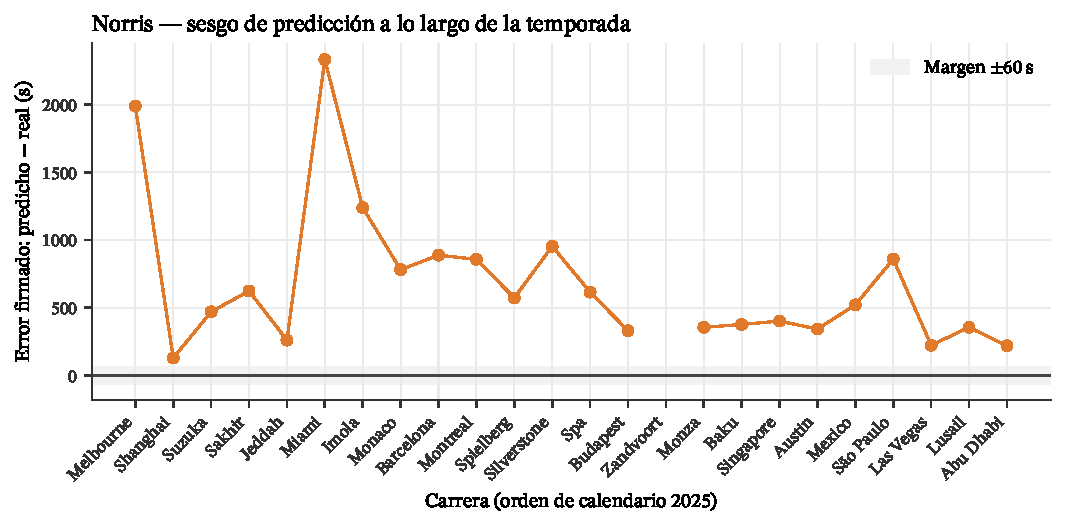
\includegraphics[width=0.9\linewidth,height=0.185\textheight,keepaspectratio]{Chapter5/images/error_signed_NOR.pdf}%
  }{\rule{0pt}{3cm}}
\end{subfigure}

\vspace{0.4em}

\begin{subfigure}[t]{\textwidth}
  \centering
  \IfFileExists{Chapter5/images/error_signed_PIA.pdf}{%
    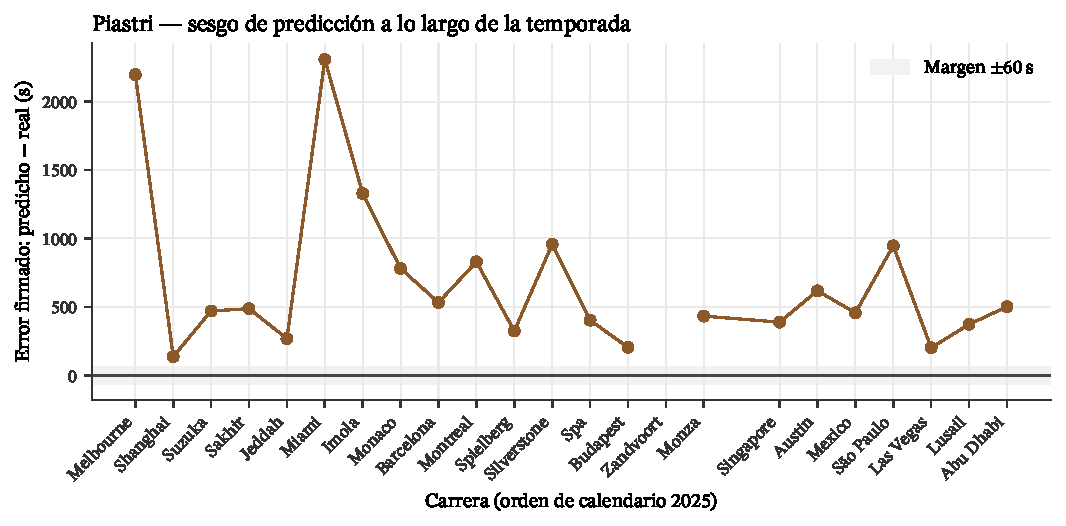
\includegraphics[width=0.9\linewidth,height=0.185\textheight,keepaspectratio]{Chapter5/images/error_signed_PIA.pdf}%
  }{\rule{0pt}{3cm}}
\end{subfigure}

\vspace{0.4em}

\begin{subfigure}[t]{\textwidth}
  \centering
  \IfFileExists{Chapter5/images/error_signed_VER.pdf}{%
    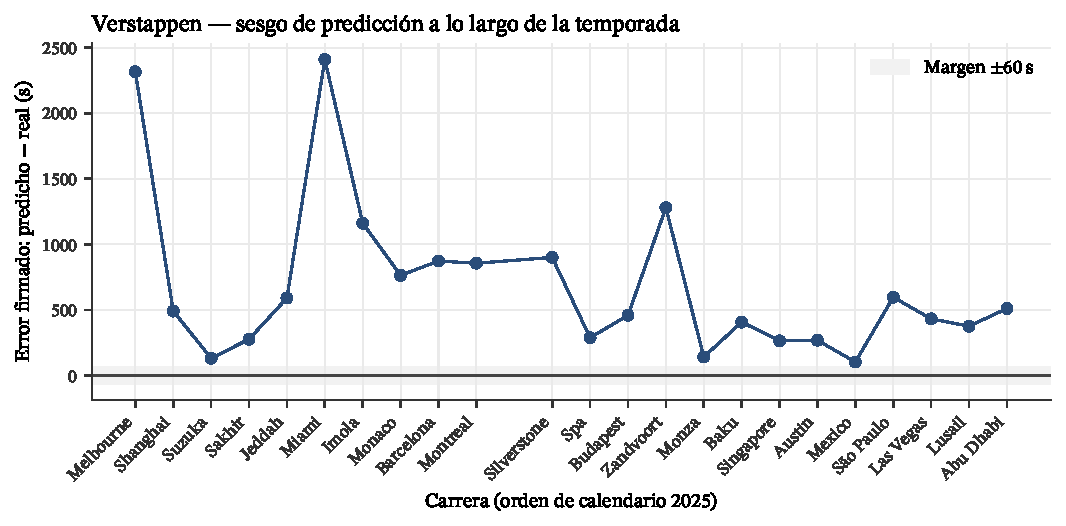
\includegraphics[width=0.9\linewidth,height=0.185\textheight,keepaspectratio]{Chapter5/images/error_signed_VER.pdf}%
  }{\rule{0pt}{3cm}}
\end{subfigure}

\vspace{0.4em}

\begin{subfigure}[t]{\textwidth}
  \centering
  \IfFileExists{Chapter5/images/error_signed_LEC.pdf}{%
    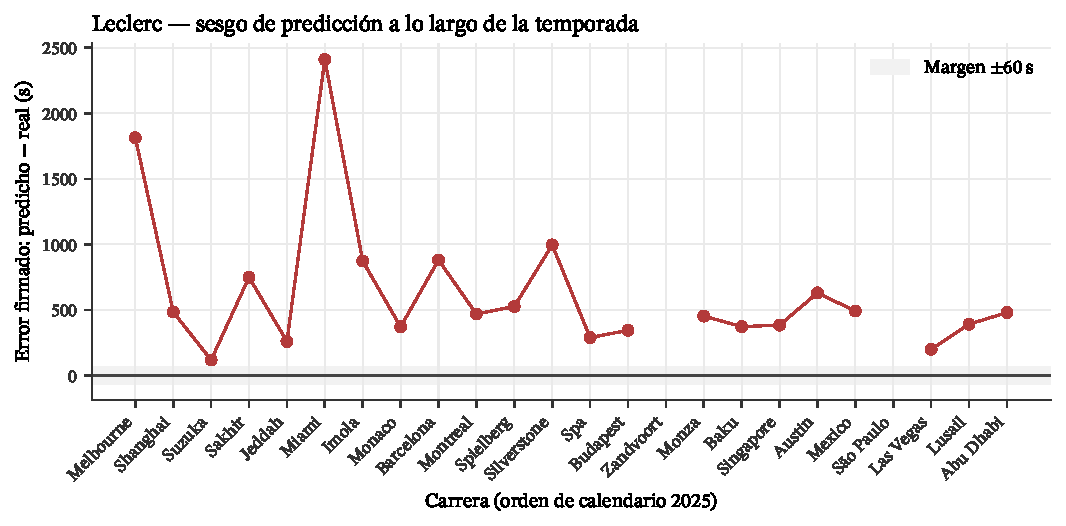
\includegraphics[width=0.9\linewidth,height=0.185\textheight,keepaspectratio]{Chapter5/images/error_signed_LEC.pdf}%
  }{\rule{0pt}{3cm}}
\end{subfigure}
\caption{Series temporales del error firmado predicho\,$-$\,real por piloto sobre las carreras evaluadas de 2025. En cada panel la franja gris marca el margen $\pm$\SI{60}{\second} aplicado por el motor frente a un evento de \textit{safety car}.}
\label{fig:eval_error_signed_all}
\end{figure}

% ──────────────── Dumbbells a página completa ────────────────
\clearpage
\begin{figure}[H]
\centering
\IfFileExists{Chapter5/images/dumbbell_NOR.pdf}{%
  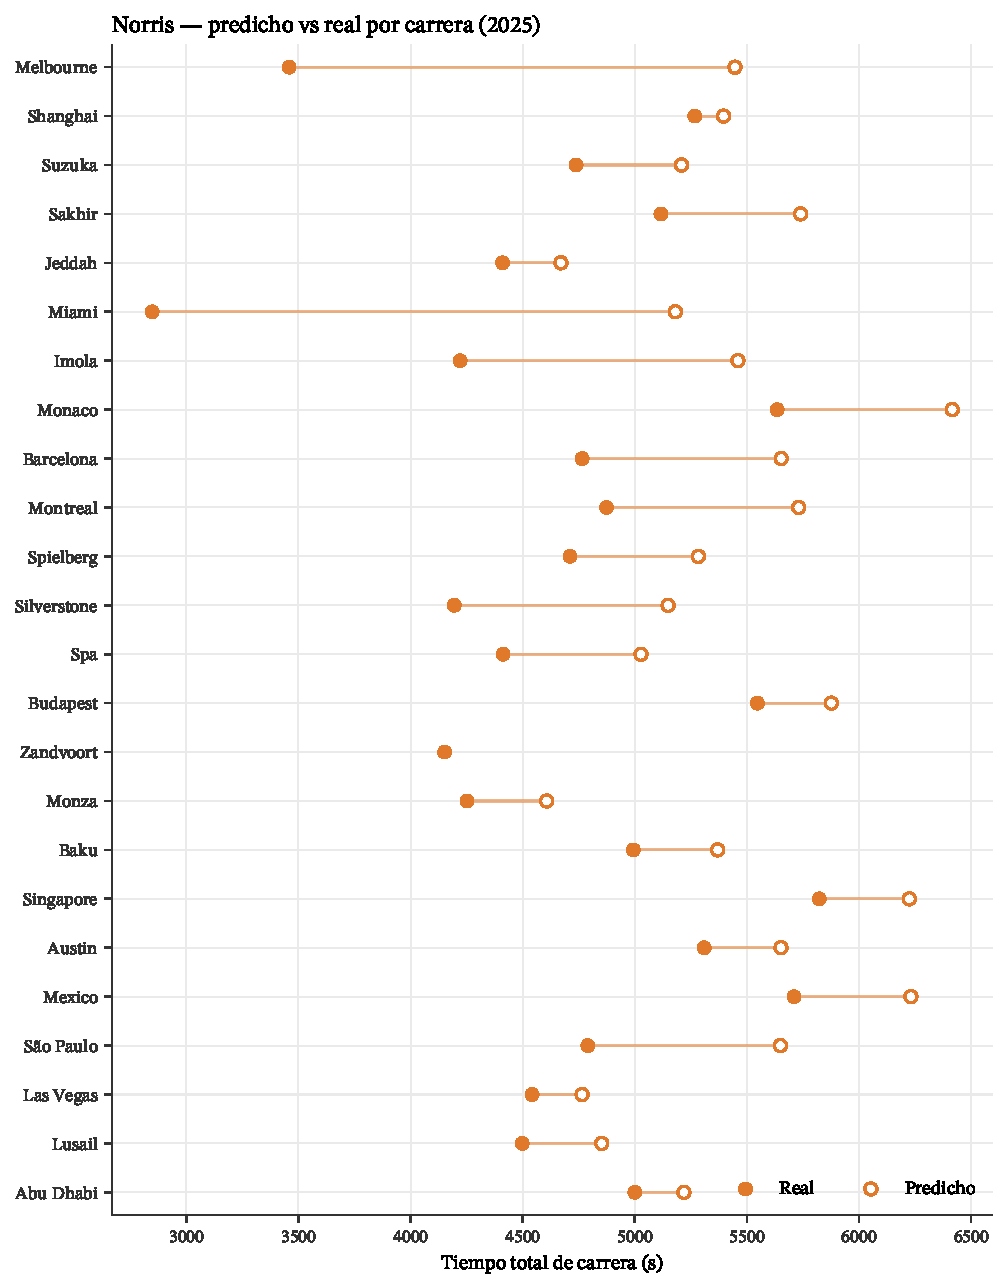
\includegraphics[height=0.85\textheight,keepaspectratio]{Chapter5/images/dumbbell_NOR.pdf}%
}{\rule{0pt}{5cm}}
\caption{Norris: tiempo predicho (círculo blanco) frente al tiempo real (círculo relleno) carrera a carrera, con el error firmado anotado a la derecha.}
\label{fig:eval_NOR_dumbbell}
\end{figure}

\clearpage
\begin{figure}[H]
\centering
\IfFileExists{Chapter5/images/dumbbell_PIA.pdf}{%
  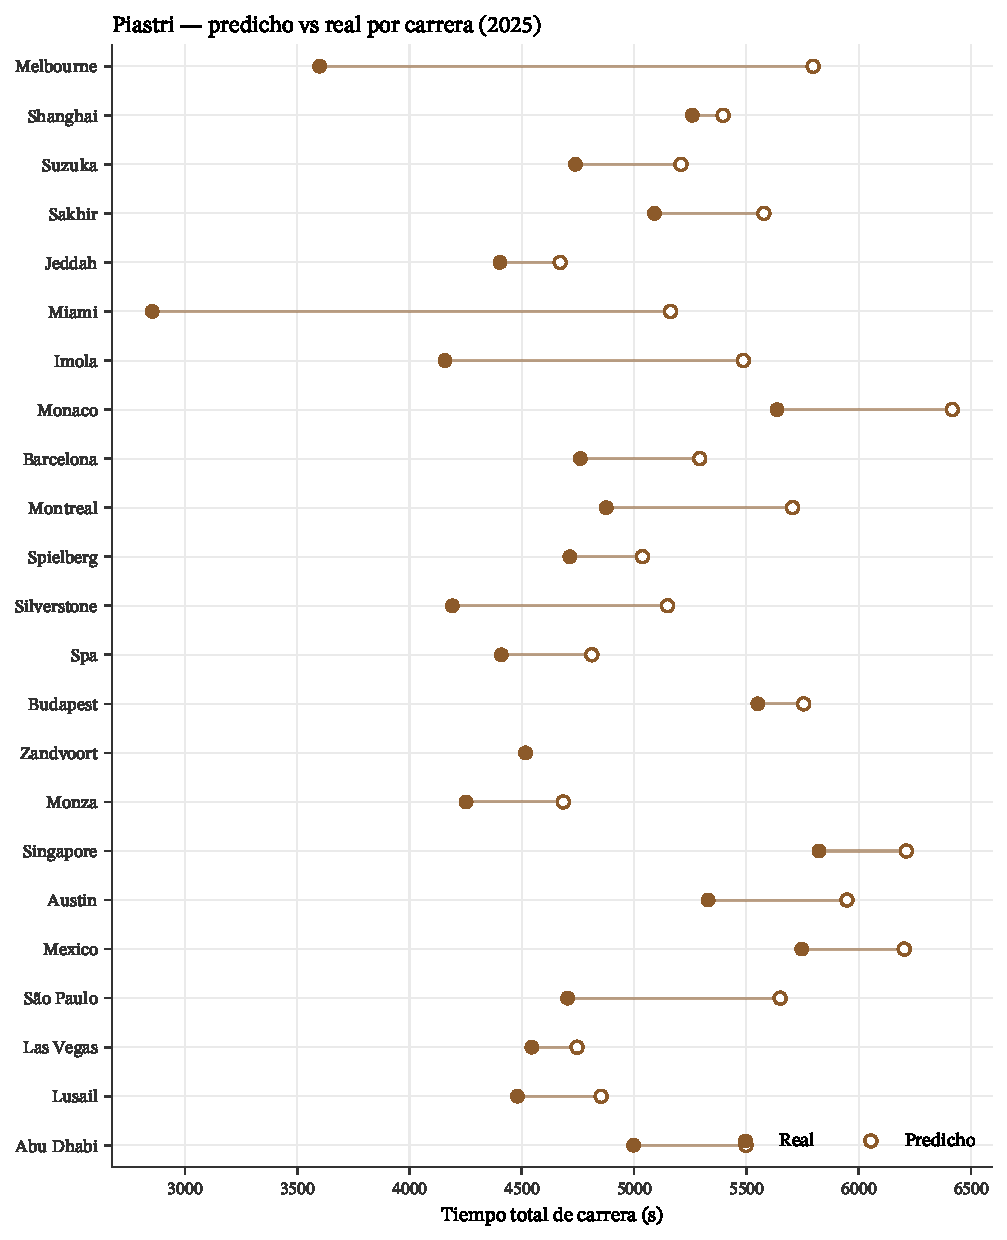
\includegraphics[height=0.85\textheight,keepaspectratio]{Chapter5/images/dumbbell_PIA.pdf}%
}{\rule{0pt}{5cm}}
\caption{Piastri: tiempo predicho frente al tiempo real carrera a carrera, con el error firmado anotado a la derecha.}
\label{fig:eval_PIA_dumbbell}
\end{figure}

\clearpage
\begin{figure}[H]
\centering
\IfFileExists{Chapter5/images/dumbbell_VER.pdf}{%
  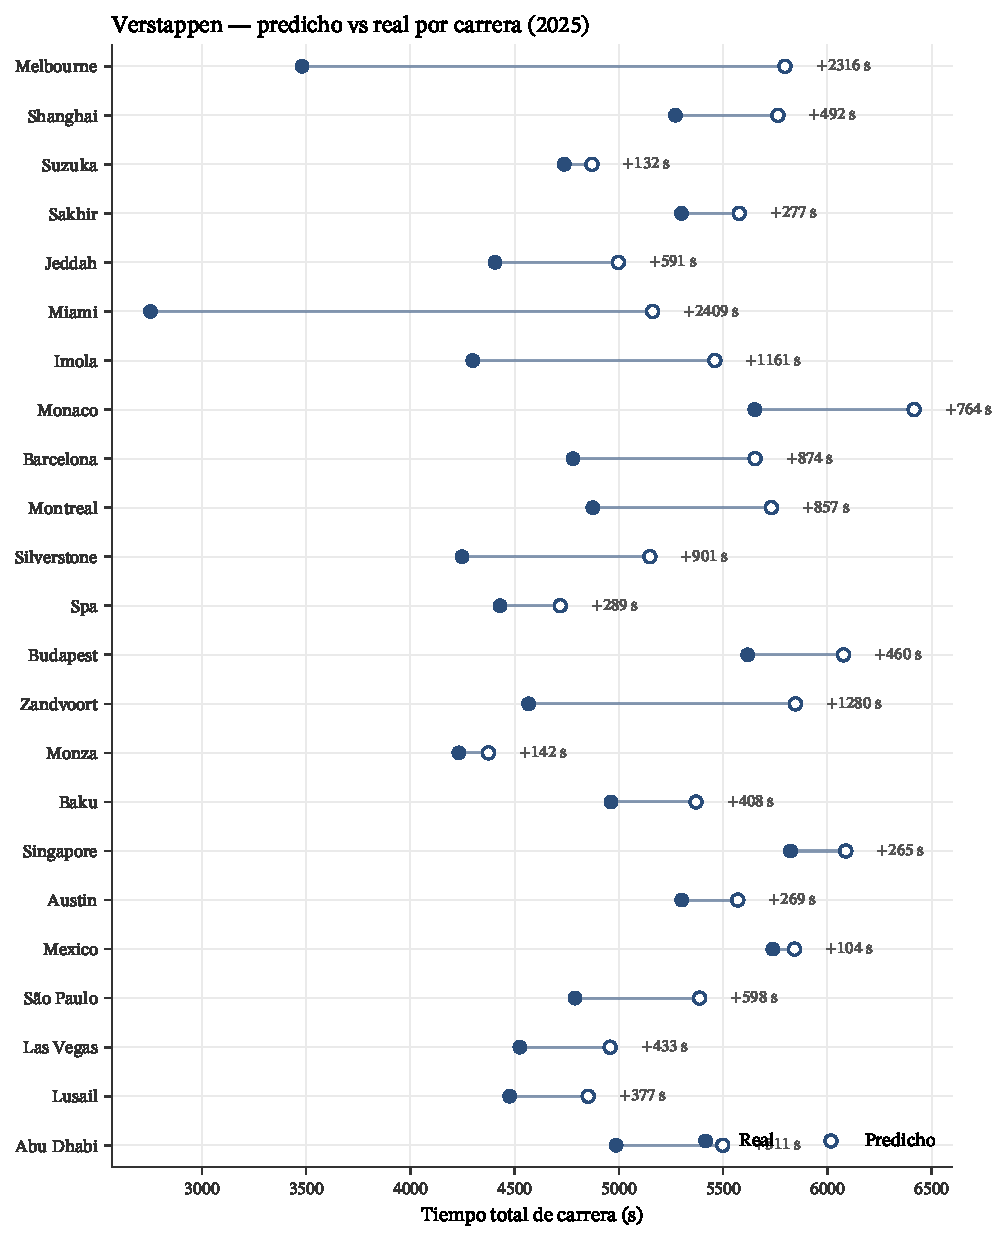
\includegraphics[height=0.85\textheight,keepaspectratio]{Chapter5/images/dumbbell_VER.pdf}%
}{\rule{0pt}{5cm}}
\caption{Verstappen: tiempo predicho frente al tiempo real carrera a carrera, con el error firmado anotado a la derecha.}
\label{fig:eval_VER_dumbbell}
\end{figure}

\clearpage
\begin{figure}[H]
\centering
\IfFileExists{Chapter5/images/dumbbell_LEC.pdf}{%
  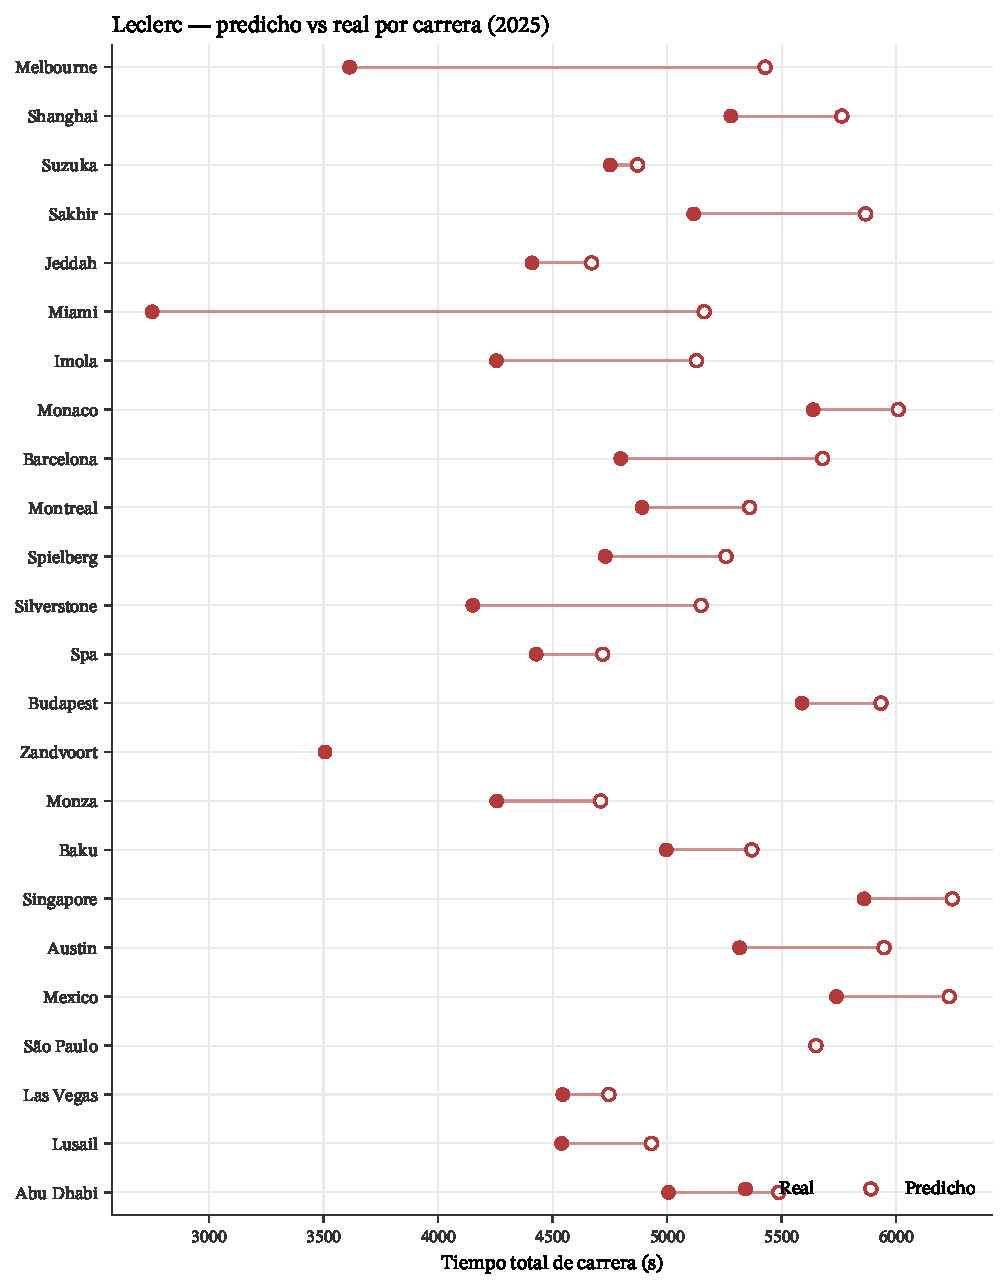
\includegraphics[height=0.85\textheight,keepaspectratio]{Chapter5/images/dumbbell_LEC.pdf}%
}{\rule{0pt}{5cm}}
\caption{Leclerc: tiempo predicho frente al tiempo real carrera a carrera, con el error firmado anotado a la derecha.}
\label{fig:eval_LEC_dumbbell}
\end{figure}

\cleardoublepage

\backmatter
\end{document}
